%=====================================================================
% Document Style
%=====================================================================
% Choose only one of the following document classes:
%
% for a 12 Point UW PhD Thesis without Margin Check
% \documentclass[12pt]{withesis}
%
% for a 10 Point UW PhD Thesis with Margin Check
%\documentclass[10pt,margincheck]{withesis}
%
% The margincheck option flags lines which overflow their hbox with a black
%  box at the end of the line.  This usually (but not always) indicates a
%  margin violation on the right margin.  Left margin violations aren't
%  indicated and if the margin violation is large enough, there isn't room
%  for the black box to be visiable.  
%
% This option can be also used in conjunction with the msthesis option.
%
% or for a 12 Point UW Masters Thesis
\documentclass[12pt,msthesis]{withesis}
%
% or for a 10 Point UW Masters Thesis
%\documentclass[10pt,msthesis]{withesis}
%
% The msthesis option changes the page margins from 1" all around
% (the PhD format) to 1.25" left and 1" remaining margins (MS format).
% The defaults for degree and thesis are changed to be MS and thesis.
% These defaults can be overridden if the margins for the MS thesis
% are desired for other documents.

% To include optional packages, use the \usepackage command.
%  The package epsfig is used to bring in the Encapsulated PostScript
%    figures into the document.
%  The package times is used to change the fonts to Times Roman; however
%    because the times typewriter font looks odd, the original LaTeX
%    Computer Modern font is kept for the typewriter font using
%      \renewcommand{\ttdefault}{cmtt}
%    Note that Times Roman is a PostScript font and therefore, the document
%    cannot be correctly viewed from the *.dvi file.  It should be converted
%    to a *.ps file first and then viewed with a PostScript previewer...

\usepackage[margin=1.5in]{geometry}     % set the margins to 1in on all sides
\usepackage{graphicx}             		 % to include figures
\usepackage{amsmath}               		 % great math stuff
\usepackage{amsfonts}              	   % for blackboard bold, etc
\usepackage{amsthm}                		 % better theorem environments
\usepackage{times}
\usepackage{epsfig}
\usepackage{multirow}
\usepackage{url}
\usepackage{algorithm}
\usepackage{algorithmic}
\usepackage{enumitem}
\renewcommand{\ttdefault}{cmtt}

% Algorithm overrides
\renewcommand{\algorithmicrequire}{\textbf{Given:}}
\renewcommand{\algorithmiccomment}[1]{// #1}

\renewcommand{\topfraction}{0.9}	% max fraction of floats at top
    \renewcommand{\bottomfraction}{0.8}	% max fraction of floats at bottom
    %   Parameters for TEXT pages (not float pages):
    \setcounter{topnumber}{2}
    \setcounter{bottomnumber}{2}
    \setcounter{totalnumber}{4}     % 2 may work better
    \setcounter{dbltopnumber}{2}    % for 2-column pages
    \renewcommand{\dbltopfraction}{0.9}	% fit big float above 2-col. text
    \renewcommand{\textfraction}{0.07}	% allow minimal text w. figs
    %   Parameters for FLOAT pages (not text pages):
    \renewcommand{\floatpagefraction}{0.7}	% require fuller float pages
	% N.B.: floatpagefraction MUST be less than topfraction !!
    \renewcommand{\dblfloatpagefraction}{0.7}	% require fuller float pages

%========================================================================
%  Draft Control Commands:
%========================================================================
%
% \psdraft causes the \psfig or \epsfig commands to draw a box and label
% the box with the postscript file name instead of reading in the full
% postscript figure.  This can save time and toner when printing drafts.
%
%\psdraft
%
%
% \psfull causes the inclusion of the postscript figures.
%\psfull
%
%
%\pagestyle{thesisdraft} causes the footer text to become:
% DRAFT: Do Not Distribute        <time><Date>        <input file name>
%
%\pagestyle{thesisdraft}
%
\pagestyle{thesis} %causes the header and footers to be the correct format
%
%\pagestyle{thesisdraft}
%
%
%  The page margins can be marked with a post-script box using the
%  \draftmargins command.  This command uses dvips's end-of-page hook
%  This is only visible in the *.ps file (NOT the *.dvi file)!
%
%\draftmargins
%
%
%  The word ``DRAFT'' can be diagonally printed across the page using
%  the \draftscreen command.  This command uses dvip's beginning-of-page
%  hook.  This is only visible in the *.ps file (NOT the *.dvi file)!
%	
%\draftscreen


%=======================================================================
% Remove the following lines if appendix tables or figures are present.
% The suppress writing the auxiliary information which appears in the
% list of tables or list of figures.
%
%\noappendixtables                % Don't have appendix tables
%\noappendixfigures               % Don't have appendix figures

\DeclareMathOperator*{\argmax}{arg\,max}

%=======================================================================
% End of Preamble, start of document
%


\begin{document}

	% Choose your bibliography style
	% plain is the basic style, others include ieeetr, siam, asm, etc
	\bibliographystyle{ieeetr}

	\clearpage\pagenumbering{roman}

\title{Massively Parallel Reinforcement Learning With an Application to Video Games}
\author{Tyler Goeringer}
\date{}
\advisorname{Soumya Ray}
\department{Electrical Engineering and Computer Science}
\maketitle


\committeechair{Soumya Ray}
\committeeb{Michael Lewicki}
\committeea{Swarup Bhunia}
\committeec{Frank Merat}
\committeeapprovalpage

\begin{acknowledgments}
First and foremost I would like to thank my adviser Dr. Soumya Ray. When I approached him with my research topic he was enthusiastic and supportive. When I encountered problems he provided advice and guidance which has made this research possible. From the start to the finish, this research would not have been possible without him.
    
I would like to thank my boss, Chris, for supporting me and approving the time off I needed to work on research. In addition I give my thanks to all those who provided technical assistance: Simon, for helping me understand the CUDA API and how to best utilize it; Thomas and Tyler, my coworkers who answered an endless stream of C\textbackslash C++ questions; and Hitesh, my coworker who provided advice on integrating into the Quake III engine.

Last but not least, I would like to express my gratitude to my parents and my sister. They have supported me in my endeavors for as long as I can remember, even when I did not acknowledge it. Without their support I would not have made it to Case and started the path that has lead me here.
\end{acknowledgments}

\tableofcontents
\listoftables
\listoffigures

\begin{abbreviations}
    Abbreviations will go here.
\end{abbreviations}

\begin{umiabstract}
    We propose a framework for periodic policy updates of computer controlled agents in an interactive scenario. We use the graphics processing unit (GPU) to accelerate an offline machine learning algorithm which periodically updates an online agent's policy. The main contributions of this work are the use of GPU acceleration combined with a periodic update model to provide reinforcement learning in a performance constrained environment. We show empirically that given certain environment properties, the GPU accelerated implementation provides better performance than a traditional implementation utilizing the computer processing unit (CPU). In addition, we show that while an online machine learning algorithm can function in some performance constrained environments, an offline algorithm reduces the performance constraints allowing for application to a wider variety of environments. Finally, we demonstrate combining these techniques to control an agent in the world of Quake III Arena, resulting in a computer controlled agent capable of adapting to different opponents.
\end{umiabstract}

\clearpage\pagenumbering{arabic}
	
	\chapter{Introduction}

The advent of general purpose programming on the graphics programming unit (GPU), commonly referred to as GPGPU, has led to a dramatic shift in the way computers are used to solve problems. In June 2010 the organization Top 500, which maintains a ranking of the top 500 fastest supercomputers, ranked a GPU based system in the \#2 spot, the first time any GPU based system had reached the top 10 \cite{top500:2010}. In June 2011 three GPU based systems were in the top 10, and in November 2012 the supercomputer Titan took the \#1 spot using 18,688 nVidia GPUs \cite{top500:2011} \cite{top500:2012}.

The high availability of discrete GPUs and the ease of development provided by GPGPU APIs have helped provide access to massively parallel programming at all levels, not just in the realm of supercomputing. Consumer applications such as Adobe Premiere \cite{adobe} and Blender \cite{blender} are also taking advantage of GPGPU to improve performance. A software development kit called PhysX is used by game developers to move physics calculations onto the GPU for more realistic rendering \cite{physx}.

The key benefit of GPGPU is the switch from serial to massively parallel processing, allowing algorithms working with large and complex data sets to operate much more efficiently. Artificial intelligence (AI) algorithms stand to benefit from this paradigm shift, allowing for more complex algorithms and better performance in existing algorithms. This, in turn, benefit AI applications such as large data analysis problems, virtual assistants, and natural language processors. However, to take advantage of these benefits algorithms must be designed with the compute constraints imposed by the GPU architecture in mind.

Reinforcement learning is a class of maching learning algorithms that works by rewarding good behavior, reinforcing policies that lead to the maximum reward. Reinforcement learning algorithms are very well studied, are applicable to a wide variety of problems, and have a low barrier to entry for developers. With this in mind, we choose to focus our efforts on the benefits of massively parallel reinforcement learning. To demonstrate the benefits we need an environment which places strict performance constraints on the AI algorithm in addition to functional design requirements. For this purpose we choose the video game Quake III.

Quake III is a first person shooter in which the computer controls agents which oppose the human player. The computer agents are expected to compete with human players ranging from novices to experts. In addition, the agents also must have unique, human-like personalities. In addition to design constraints, AI agents in Quake III are heavily performance constrained. A common number given for the amount of time available for making a single decision is $1-3$ ms \cite{game:ai:lecture}. This number comes from the assumption that a single frame of video for the game takes $33$ ms and the AI accounts for around ten percent of this calculation. In reality, many AI calculations are done across multiple frames to get around this performance constraint. Even if we amortize over the course of one second, all of the game's AI agents have around $90$ ms to make decisions.

We demonstrate the use of hardware acceleration and iterative update off-line reinforcement learning as a solution to the performance constraints in video game AI. Hardware acceleration allows certain algorithms to perform faster than traditional computation by an order of magnitude or more. We believe combining this speed increase with a policy which is periodically updated by a background process will allow more realistic automated agents to funtion in a wide vareity of performance constrained environments.
	\chapter{Background}
\label{chap:background}

In this chapter we provide some background on the MDP framework, which is the representation of the problem used by our algorithms to obtain agent policies. We then describe reinforcement learning and the basic policy iteration algorithm, followed by a discussion of GPU architectures and general purpose programming on the GPU.

\section{Markov Decision Process}

A \emph{Markov Decision Process} (MDP) \cite{norvig} is a specification of a sequential decision process in a fully observable environment with five components. An MDP can be represented by the 5-tuple $(\mathcal{S, A, P}, R, \gamma)$ where: $\mathcal{S} = \{s_1, s_2, ..., s_n\}$ is a finite set of states; $\mathcal{A} = \{a_1, a_2, ..., a_m\}$ is a finite set of actions; $\mathcal{P}$ is a Markovian transition model where $\mathcal{P}(s, a, s')$ is the probability of making a transition to state $s'$ when taking action $a$ while in state $s$; $R$ is a reward function such that $R(s, a, s')$ is the reward for the transition represented by $(s, a, s')$; and $\gamma \in [0, 1)$ is a discount factor for future rewards.

The solution to an MDP is a \emph{policy}, denoted by $\pi$. Given the stochastic nature of an MDP, a given policy is rated based on the expected utility, as measured by $R$, of actions selected by the policy. The optimal policy for a given MDP is the policy which yields the highest expected utility and is denoted by $\pi^*$. An agent following policy $\pi^*$ acts by determining the current state $s$, and executing the action specified by $\pi^*(s)$.

When defining the expected utility of an MDP, the horizon must first be described as finite or infinite. A finite horizon occurs when there is a fixed time $N$ after which actions have no effect on reward or cost. An infinite horizon does not have any fixed limitation. With an infinite horizon the optimal policy is stationary; that is, $\pi^*(s)$ is independent of time. With a finite horizon the optimal policy changes over time and is described as non-stationary. We assume all MDPs have an infinite horizon.

Given an MDP with infinite horizon the utility of a state sequence can be defined as either additive or discounted. For additive rewards the utility of a state sequence is:
\[
    U_h([(s_0,a_0),(s_1,a_1),(s_2,a_2),...]) = R(s_0,a_0,s_1) + R(s_1,a_1,s_2) + R(s_2,a_2,s_3) + ...
\]
For discounted rewards the utility of a state sequence is:
\[
    U_h([(s_0,a_0),(s_1,a_1),(s_2,a_2),...]) = R(s_0,a_0,s_1) + \gamma R(s_1,a_1,s_2) + \gamma^2 R(s_2,a_2,s_3) + ...
\]
The discount factor $\gamma$ is defined as a number between $0$ and $1$. From this it is clear that additive rewards is a special case of discounted rewards with $\gamma = 1$.  Note that as $\gamma$ approaches $0$, the utility function becomes weighted toward immediate rewards and as $\gamma$ approaches $1$ the utility function becomes weighted toward long term rewards. We assume all MDPs use discounted rewards with $\gamma \in [0, 1)$.

\section{Policy Iteration}

Given a complete model, $(\mathcal{S, A, P}, R, \gamma)$, of an MDP it is possible to use the policy iteration algorithm to determine an optimal policy. The policy iteration algorithm requires some initial policy $\pi_0$ followed by the repeated iteration of two steps: policy evaluation and policy improvement \cite{norvig}. Policy evaluation calculates the utility of policy $\pi_i$ such that $U^{\pi_i} = U_i$ where 
\[
    U^{\pi_i} = R(s_0,\pi(s_0)) + \gamma R(s_1,\pi(s_1)) + ...
\] 
Policy improvement computes a new policy based on $U_i$ in an attempt to improve on policy $\pi_i$. These two steps are repeated until the policy improvement step no longer yields a change in the utilities: $U_i \approx U_{i+1}$.

To confirm that this results in an optimal policy, we must examine how the utility function is generated during each iteration. For compact notation let $R(s,a)$ be the weighted sum of rewards over $s'$:
\[
    R(s,a) = \sum_{s' \in S} \mathcal{P}(s,a,s')R(s,a,s')
\]
Assuming the goal is to maximize the utility, the optimal policy can be defined using Equation \ref{eq:opt:policy}.
\begin{equation}
    \pi^*(s) = \argmax_a \sum_{s'} \mathcal{P}(s,a,s')U^*(s')
    \label{eq:opt:policy}
\end{equation}

The maximum utility of a state satisfies the Bellman optimality criterion:
\[
    U^*(s) = R(s,a) + \gamma \max_a \sum_{s'}\mathcal{P}(s,a,s')U^*(s')
\]
This function is derived from the idea that the utility of each state is equivalent to the reward at that state plus the sum of the discounted rewards of all following states. For an MDP with $n$ states there are $n$ Bellman equations and $n$ unknowns (the utilities of the states). Optimizing the Bellman criterion provides an optimal policy. One way to do this is to use dynamic programming and the Bellman update:

\begin{equation}
    U_{i+1}(s) \gets R(s,a) + \gamma \max_a \sum_{s'}\mathcal{P}(s,a,s')U_i(s')
    \label{eq:bellman:update}
\end{equation}

The utility function $U_i$ which results from policy iteration is a fixed point of the Bellman update, which means it is a solution to the Bellman optimality criterion and thus $\pi_i$ must be an optimal policy.

To perform the policy evaluation step we can use the Bellman equation:
\begin{equation}
    U_i(s) = R(s,a) + \gamma \sum_{s'} \mathcal{P}(s, \pi_i(s), s')U_i(s')
    \label{eq:bellman:eval}
\end{equation}

The optimal policy can now be determined using Equation \ref{eq:bellman:eval} to determine $U_i(s)$ for all $s \in S$ and using Equation \ref{eq:bellman:update} to generate $\pi_{i+1}(s)$.

\section{Reinforcement Learning}

Policy iteration requires the complete model of the underlying MDP. However, in practical control problems it is often the case that a complete model is not available \cite{lspi}. Most commonly, the transition model and reward function are unknown. To solve these problems we need agents which can learn optimal policies through the process of reinforcement learning. A typical reinforcement agent will generate a policy by acting within the environment and use positive and negative outcomes to reinforce good policy decisions and avoid bad policy decisions.

The observations of an agent acting in an environment can be organized in tuples referred to as samples: $(s, a, r, s')$. This sample layout means the agent was in state $s$, took action $a$, received reward $r$, and ended up in state $s'$. These samples can be collected by interacting with the environment or by using a simulation of the environment.

\subsection{Online and Offline Reinforcement Learning}

An online reinforcement learning agent is one which performs policy updates while actively interacting with the environment. A typical online reinforcement learning agent will start with some initial policy and interact with the environment by either selecting an action at random or following the current policy. The proportion of time the agent spends randomly selecting an action is the exploration rate. Changing the exploration rate will affect the policy generated by shifting toward or away from local maximums. An agent with a very low exploration rate is likely to generate a policy based on the earliest successful actions it takes, while an agent with a very high exploration rate may take longer to converge to a policy but is more likely to explore the entirety of the state-space. Some agents use more advanced exploration policies in an attempt to explore the state-space more effectively.

In contrast, an offline reinforcement learning agent generates a policy without directly interacting with the environment. Generally this is achieved by using existing samples from the environment or a simulation. Because offline agents do not directly interact with the environment they do not have control over exploration policy in the environment. This can be limiting; however, this also provides a high level of flexibility as there are no restriction on how the samples are gathered. For example, an offline agent can trivially generate a policy based on the experience of an existing agent or even multiple existing agents. With online agents this is usually not possible, although an existing online agent can provide a starting policy for another agent.

A key benefit of offline agents is the decoupling of action selection and policy updates. As a result, offline algorithms generally guarantee convergence in the presence of approximate models. In addition, decoupling the action selection from policy updates reduces the number of operations necessary for an agent to make decisions. 

In video games action selection decoupling is particularly important as agents have a very strict time restrictions. Video game agents are expected to act at least as often as graphics are drawn to the screen. Using a minimum framerate of 30 hertz results in a maximum decision time of 33 ms \cite{game:ai:lecture}. When an online agent selects an action, it is also required to perform a policy update step. Because of this requirement it may be unfeasible to use online agents in a video game; however, an offline agent may be more feasible because the policy update step is decoupled from interacting with the environment.

\section{General Purpose Programming on the GPU}

In the early 1990s the central processing unit (CPU) was responsible for almost the entirety of processing on a desktop computer system, including the video output. Following the advent of graphical operating systems, demand for better visual processing applications increased at a rate which performance increases on the CPU could not sustain while still providing a responsive user experience. In response a domain specific piece of hardware was created, the graphics processing unit (GPU). Today the architecture of the GPU has allowed expanded to general purpose programming in support of high performance computing applications. This section will provide an overview of the architecture of the GPU, compare it to that of the CPU, and explain the advent of general purpose programming on the GPU (GPGPU).

\subsection{CPU Architecture}

CPUs were originally designed to process only one task at a time and performance improvements were focused heavily on improving the speed at which a series of calculations could be performed. At the most basic level a CPU consists of a fetch and decode unit, an execution unit, and a set of registers. Fetching and decoding units pull the next instruction set for a program and orchestrate the calculations. The calculations themselves occur in the execution unit, and the registers store the data needed for execution \cite{gpgpu}. This minimal processor architecture is displayed on the left in Figure \ref{fig:cpu}.

\begin{figure}
    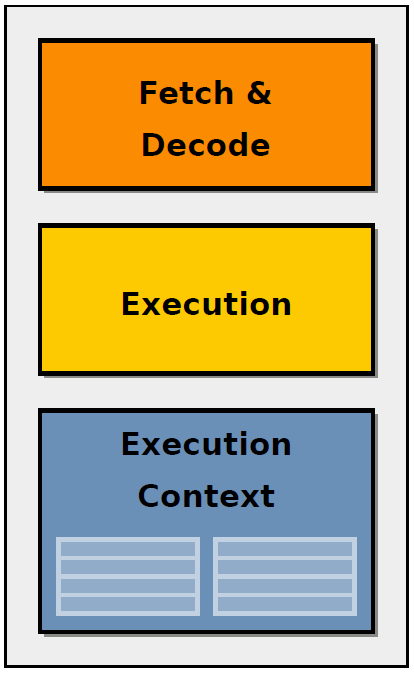
\includegraphics[height=0.25\paperheight]{CPU_Simple.png}
    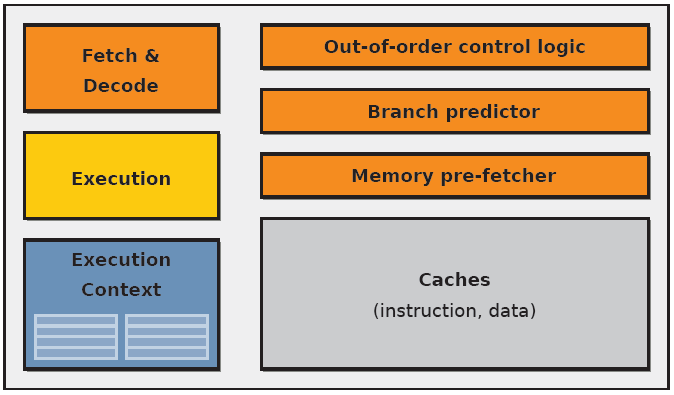
\includegraphics[height=0.25\paperheight]{CPU.png}
    \caption{Processor architecture diagrams. Left: A minimally functional processor. Right: A modern CPU. \cite{gpgpu}}
    \label{fig:cpu}
\end{figure}

This basic CPU design, however, has many speed limitations. Fetching instructions and data from main memory is an expensive operation and some of the execution units may spend time idle depending on the program flow. Many performance optimizations are used to reduce the impact of these limitations. Out-of-order execution allows instructions to be re-ordered to use execution units in parallel, memory is pre-fetched based on what data is expected to be needed by the next set of instructions, and the CPU will predict which branch will be taken by a program. These optimizations all improve the throughput offered by a single instruction stream.

Modern CPUs also take advantage of the knowledge that multiple instruction streams are all trying to execute simultaneously. If one stream stalls or does not fully utilize the execution units, the CPU will try to use idle units to begin calculations for an instruction set from a different stream. These changes, demonstrated in Figure \ref{fig:cpu}, facilitate higher performance for programs which separate programming instructions into multiple threads.

More recently, CPUs have moved to low levels of parallelization as well. Rather than increasing the speed of a single instruction stream, new models will duplicate hardware to support completely simultaneous execution of multiple instruction streams.

\subsection{GPU Architecture}

Due to the nature of computer graphics, GPUs were designed to focus on parallelization rather than single stream throughput. Graphical scenes are generally represented as a large number of discrete parts, each of which must be processed using a single transformation. These transforms can usually be applied to each discrete part independently of the rest of the scene. In order to process as many portions of the scene at once, a high number of basic processors is required \cite{gpgpu}.

GPUs require the same basic architecture as the CPU: a fetch and decode unit, an execution unit, and registers. Using this simple design does not provide the same throughput per stream as the more advanced CPU design, but it allows more processing cores to be included on the same chip to support many parallel streams. However, just as the CPU design became optimized for single streams, the GPU design was optimized for multiple streams.

Suppose we use an image editing program to change the hue of a picture with dimensions of 1280x1024. This picture has 1,310,720 individual pixels, each of which must be processed using the same linear transform. With a single core CPU this operation would need to be repeated for each of these pixels. If we use a GPU with 32 processing cores we could reduce the number of operations required to 40960.

Reducing the operations by using 32 processing cores is helpful, but would still be a slow process, particularly for more complicated transformations. Luckily, the GPU can optimize this operation further by taking advantage of the fact that each pixel is undergoing the same instructions. This optimization, demonstrated in Figure \ref{fig:simd} is called single instruction, multiple data (SIMD) processing. Rather than using a fetch and decode unit for every instruction stream, multiple registers and execution units share the same fetch and decode unit.

\begin{figure}
    \centering
	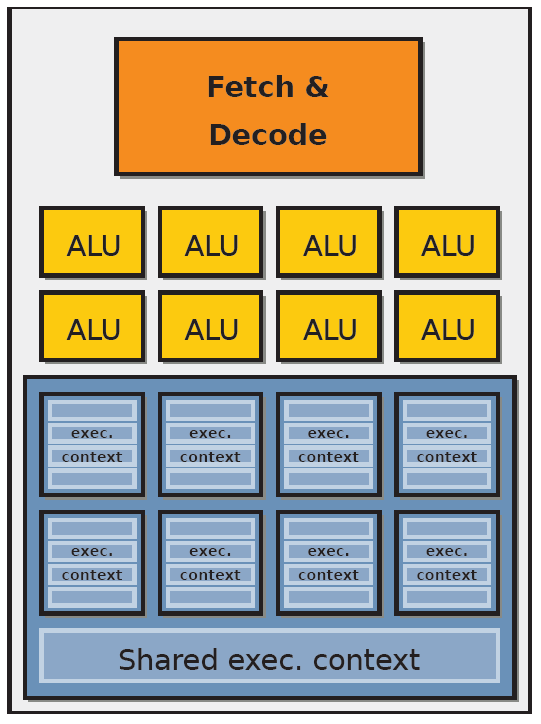
\includegraphics[height=0.25\paperheight]{SIMD.png}
    \caption{The SIMD architecture. \cite{gpgpu}}
	\label{fig:simd}
\end{figure}

Using SIMD processing the GPU is able to scale to very large number of simultaneous streams without requiring as much hardware. Now imagine that each of our 32 processing cores has 8 execution units and 8 registers. The calculation can now be completed in 5120 steps, a factor of 256 speedup! This performance boost does have one drawback: each of the processing cores must perform the same instruction across all execution units. This has some implications for GPGPU which will be discussed in the next section.

\subsection{Programming Model}

There are two main approaches to making the GPU's SIMD architecture available to programmers: explicitly using vector instructions, or implicitly using threads. Explicit instructions require the code to be written specifically for use on a GPU architecture. This can be beneficial as it requires the developer to carefully design algorithms for use on the GPU. However, manually writing highly parallelizable code can be difficult and hardware specific, thus reducing portability and requiring more development time \cite{gpgpu}.

Implicit models allow for programmers to write code as if it were for any multi-threaded CPU architecture. This can make the transition from CPU to GPU programming easier, but it also makes it easier to write very inefficient code. Despite the model allowing operations to be programmed using threads, groups of threads still must share the same fetch and decode unit. If the programmer is not aware of this limitation, it is possible to write code which attempts to branch threads operating on a single SIMD, lowering performance.

Unlike the CPU, the GPU does not have a sophisticated memory caching hierarchy. This is because graphical applications tend to share the same data across multiple execution units. Instead, the GPU memory architecture focuses on high bandwidth for transferring large amounts of data. As a result, random memory access suffers from high latency which can reduce performance. To overcome this problem for GPGPU solutions, a small cache of local memory is usually accessible. However, this cache is generally very small and so programmers are relied upon to write code that minimizes the need for random memory access.

In the early days of GPGPU, developers utilized the GPU by converting data input into graphical textures and defining algorithms in terms of programmable shaders. This was very difficult for some tasks which did not logically map well to graphics operations. In response, programming APIs have been developed to facilitate easier access to GPGPU. The two main APIs available today are CUDA, an nVidia specific API, and OpenCL, an open standard which is supported on both nVidia and AMD video cards \cite{gpgpu}.

    \chapter{Artificial Intelligence in Video Games}
\label{chap:games}

In video games the implementation of artificial intelligence (AI) is generally constrained most heavily by performance. Maintaining the illusion of a virtual world requires an AI agent to react within a time frame that is reasonable for a human player. Turn-based strategy games like chess or checkers are less impaired by performance because human players are often expected to take long periods of time to make a decision; however, real-time games generally require decisions to be made in milliseconds, severely limiting the complexity of the AI algorithm used. This chapter will provide a brief look at common AI techniques using concrete examples.

\section{Pac-Man}

Early computer controlled video game agents relied primarily on scripting and randomization. Scripting is a process by which a developer manually creates a set of a rules which govern an agent's actions. Randomization was often included in these rules to increase the difficulty of determining how the agent would behave, as well as to mimic human behavior which does not always follow strict rules. A famous example is Pac-man, which made clever use of scripted AI in order to create the illusion that each enemy possessed a different personality \cite{pacman}.

Pac-Man is a game in which the player controls a hungry character, known as the pac-man, who must navigate a maze in order to eat `food' while avoiding enemies called `ghosts'. The ghosts are controlled by the computer and their goal is to kill the player by touching him. They have limited speed and pac-man can consume a special item to make the ghosts vulnerable to attack for a short period of time. Over the years fans of the game Pac-Man have studied and dissected the behavior of the ghosts and published these results as ``The Pac-Man Dossier'' \cite{pacman}. This dossier goes into great detail about the behavior of the ghosts with the intent of allowing players to exploit weaknesses in their behavior.

Each ghost was given a unique set of rules to guide them, resulting in behavior that many players see as resulting from different personalities. One of the ghosts, named Blinky, was programmed to always move toward the space currently occupied by the player. As a result, this ghost was seen as more aggressive and was more likely to kill the player than the other ghosts. Another ghost, called Pinky, was programmed to always target a space in front of the player's direction of movement.

In addition to each ghost's unique movement rules, all ghosts were subject to global rules which helped to prevent the player from being hunted relentlessly. Periodically the ghosts would switch between a chase mode, during which their unique rules were in place, and a scatter mode, during which each ghost would flee to a pre-configured path.

The rules controlling the ghosts in Pac-Man can be trivially represented with conditional statements. This is the signature of scripted AI: simple, fast, and easy to control. For these reasons, scripted AI remains prevalent to this day and often serves as the building block for more complex techniques.

\section{Quake III}
\label{chap:games:quake}

Quake III is a video game in the genre of first person shooters (FPS). In Quake III the player controls a humanoid character fighting against opposing humanoids, called `bots', in arena-style combat. All players, human or bot, can pick up different weapons which each have different characteristics. Weapons spawn in pre-defined locations on the map as well as other items such as ammunition, health, and armor. Increasing health and armor improves a character's ability to survive attacks from an opponent. Each time a character dies they respawn with a default weapon and stat levels which can be improved by collecting items on the map. The goal is to kill your opponents until you reach a pre-defined kill count which signifies victory. 

The environment for Quake III is orders of magnitude more complex than that of Pac-Man. In Quake III the world is continuous, three dimensional, governed by physics which approximates reality, and the bots were designed as a stand-in for human opponents. To meet this challenge, a more complex AI system than just scripting was required. The designer of this AI, J.M.P van Waveren, designed a hierarchical system which relied on finite state machines for efficient decision making and combined this with fuzzy logic to provide unique personalities \cite{q3bot}.

\begin{figure}
	\centering
		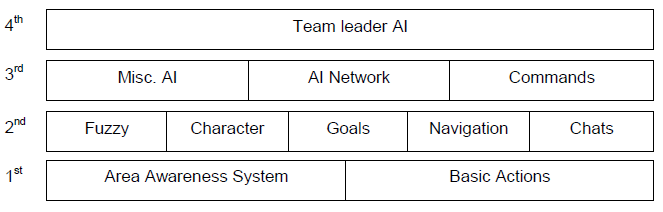
\includegraphics[width=0.80\textwidth]{q3_layers.png}
	\caption{The Quake III AI layers. \cite{q3bot}}
	\label{fig:q3:layers}
\end{figure}

The core of the Quake III bot is composed of four levels, as shown in Figure \ref{fig:q3:layers}. At the lowest level exists the area awareness system (AAS) and the basic actions interface. The AAS provides feedback on the physical state of the world around the bot, such as items or enemies which are visible. The basic actions interface provides a translation of bot commands into the same keyboard inputs a human player uses.

The second level is separated into sections for handling navigation, chat, and bot preferences. This level feeds into the third level, which directs goal-seeking behavior as well as logic to support chat commands and team communication. The fourth level is responsible for coordination between team members.

Breaking the AI design into these levels and sections drastically reduces the complexity of creating a competitive bot. Each of these sections can be designed using very simple decision making structures, but the end result is a bot which was capable of competing with the average human and even coordinating in groups. Most of these sections were implemented as straightforward conditional scripts, with two notable exceptions: the bot preference system and the \emph{AI Network}.

\subsection{Bot Preference}

The bot preference system was implemented in order to allow different bots to have different personalities. Imagine you wanted to implement a bot, Rocky, who has a particular affinity for the rocket launcher. A first attempt might simply have Rocky always go for the rocket launcher. Now imagine how Rocky would perform on a large map, if he spawned in a location such that he needed to cross the entire map in order to reach the rocket launcher. In this scenario, Rocky would have a high risk of being intercepted on the way to the rocket launcher. At this point it would become difficult for him to decide what items to pick up and what weapon to use if he decides to fight. You could start scripting the AI to handle this, but with an extremely large number of scenarios to handle scripting quickly becomes an impossible solution.

To get around this problem, Waveren implemented a fuzzy logic system \cite{q3bot}. Fuzzy logic assumes all values have some continuous truth, rather than just \emph{true} or \emph{false}. This system allows for a lot more granularity in goal selection. Going back to the previous example, rather than simply programming Rocky to go for the rocket launcher, Rocky would be given a high preference for the rocket launcher. To fully flesh out his personality, you would need to fill in his preference for other weapon types, as well as some other characteristics which would determine how likely he is to run from a fight when he does not have the upper hand.

Once Rocky's preferences are filled out, he can then make decisions based on the state of the environment and his own preferences. Now when Rocky starts out he will likely head toward the rocket launcher, but this time when he is approached by an enemy he will be capable of selecting a good nearby weapon to fight with before resuming his trek toward the rocket launcher. This preference system provides a very simple way to create a new bot personality without having to modify the code or logic. Another benefit is that Rocky will know how to behave regardless of the map, items available, or number of enemies that approach him, all without needing to set anything more than his preference values.

\subsection{AI Network}

While the preference system handles decisions regarding what weapons to pick up and what weapon to use, the bot still needs to know when it is a good idea to search for items, fight an enemy, or run away. These decisions are handled by the AI Network. Consider again the situation Rocky was in when an enemy intercepted him while he was searching for the rocket launcher. From a high-level perspective, Rocky can choose to fight, run, or pick up a nearby item. Once again, writing conditional scripts to handle this situation would result in complex code that cannot apply to new maps or item layouts.

\begin{figure}
	\centering
		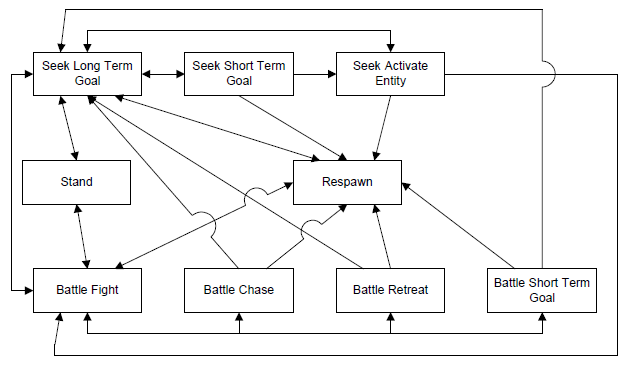
\includegraphics[width=0.80\textwidth]{q3_fsm.png}
	\caption{The Quake III AI Network. \cite{q3bot}}
	\label{fig:q3:fsm}
\end{figure}

Instead of conditional scripts, Waveren implemented the AI Network using a finite state machine as demonstrated in Figure \ref{fig:q3:fsm} \cite{q3bot}. A finite state machine consists of a number of nodes, called  `states', and edges which guide transitions between states. Rocky starts in an initial state called `Seek Long Term Goal'. In this state Rocky uses his preferences and some knowledge of the map to select a long term goal; in our scenario, that would be the rocket launcher. 

As Rocky moves around the map he evaluates the state and checks if anything matches the conditions specified on a transition from the long term goal state. If Rocky runs into an enemy, he would see there is a transition from `Seek Long Term Goal' to `Battle Fight'. Once Rocky is in this state, the transitions available to him change, as do the states he can transition into. 

On its own the finite state machine does not provide a generic decision making process, it just lowers the complexity of the implementation. However, the AI Network transitions are guided by bot preferences, generalizing the decision making process. Between the AI Network and the bot preferences, the Quake III bot provides a strong foundation for a general-purpose AI which is capable of acting in a wide variety of environments without any the need for environment specific logic.

\section{F.E.A.R.}

When F.E.A.R. was under development, the expectations for realistic bot behavior in FPS games was on the rise. Traditional techniques, such as the finite state machine in Quake III, were still resulting in complex and unmanageable behavior. In an attempt to curtail the increasing complexity, the development team decided to use planning algorithms.

A planning system works by defining a goal and a set of actions, then using an algorithm which determines what series of actions will reach that goal. Each action can be represented as a set of prerequisites and expected results. For example, the action $FireWeapon$ might have the prerequisite $WeaponEquipped \land HaveAmmo$ and the expected result $EnemyDead$.

Imagine Rocky is once again searching for a rocket launcher. When Rocky enters a room he sees an enemy at the other side of the room. Rocky checks and finds that $EnemyDead$ is a goal, and that $WeaponEquipped$ is true but  $HaveAmmo$ is false. Luckily for Rocky, a stash of ammunition is nearby and he has the action $PickupAmmo$, which has the prerequisite $AmmoNearby$ and the effect $HaveAmmo$. Rocky then plans to execute the action $PickupAmmo$ followed by $FireWeapon$. Because $FireWeapon$ does not guarantee the effect $EnemyDead$, Rocky will repeat $FireWeapon$ until he kills the enemy.

What happens if Rocky's enemy then runs? Obviously the plan Rocky formed is no longer valid. In this situation, Rocky can then re-evaluate the state of his environment and formulate a new plan to reach his goals.

F.E.A.R.'s planning system reduced the complexity of implementing well-behaved AI by decoupling decision making from the environment. To create a bot, only the actions available to the bot and the goals are needed, the remainder is handled by the planning algorithm. In addition, because the plan and state transitions are dynamically determined, the bot is capable of behavior that is not directly programmed. The end result of this system was a bot which was universally applauded for realistic, tactical bots.

\section{Reinforcement Learning in Video Games}

In the paper ``Learning Agents in Quake III'' researchers from University of Utrecht applied Q-learning to a neural network in order to train combat movements \cite{q3combat}. Neural networks are data structures used to control agent policies by using layers of nodes, each of which takes in an input, processes it, and passes the output to the next layer of nodes \cite{norvig}. Q-learning is an online reinforcement algorithm which was used to learn the optimal weights for each node \cite{norvig}.

The resulting bot was capable of defeating an identical opponent by using superior combat movements in $65\%$ of matches. However, in order to achieve these results they were required to place some restrictions on the environment: the bot was restricted to a single weapon, the room could not have any corners, and there were no obstacles. Additionally, learning the optimal weights required approximately $10$ hours of playtime. While their results were promising, the techniques they proposed are more suitable to generating a policy before letting a user play the game, rather than allowing the bot to develop better techniques while a user is playing.

In 2010, researchers Purvag Patel, Norman Carver, and Shahram Rahimi demonstrated Q-learning in a simulated FPS environment \cite{game:ai:learning}. They created a simulated environment based on the game Counter-Strike for their experiments. First they created a static AI bot which would patrol the map and then they implemented a Q-learning bot designed to learn policies to complete specific tasks, such as killing the enemy or dropping an item at a particular location.

The Q-learning bot randomly selected a patrol route and periodically checked the state to decide if it should start attacking. Further experiments were run with more complicated actions available. The result was an agent capable of learning near optimal policies after only a few thousand samples. While encouraging, because this experiment was done in a simplified and simulated environment, it is difficult to judge how effective the techniques would be when applied to the actual Counter-Strike environment.

Researchers at Lehigh University used Q-learning to generate team coordination policies for agents in the FPS Unreal Tournament, an algorithm they called RETALIATE \cite{retaliate}. The individual bots on all teams followed the same scripted behavior in order to ensure the only variable in performance was the team strategy. In addition to the RETALIATE team, they implemented three scripted teams and a team which used a technique called Hierarchical Task Network (HTN). The HTN team used dynamic planning techniques to develop their policy.

Within a single match, RETALIATE was able to easily learn policies which could defeat the scripted bots. The HTN bot proved more difficult to defeat, but RETALIATE was capable of learning an optimal policy after only two matches.

Our work differs from these experiments primarily in that it evaluates an agent executing in the Quake III environment without utilizing any simulations or restricted environments. In addition, our proposed algorithm uses the GPU to improve performance.
	\chapter{Massively Parallel Learning Algorithms}

As discussed in the background section, offline learning algorithms have the potential to provide machine learning behavior for agents acting in performance constrained environments. To demonstrate this potential we chose to us Least-Squares Policy Iteration (LSPI) and compare it to an online policy gradient algorithm. This chapter presents these algorithms in mathematical detail and suggests a modification to LSPI to support its use as an online algorithm for performance constrained environments. Some of the derivation steps of the core algorithms have been left out, for more information please see the referenced sources. Details on how we integrated these algorithms in the Quake III environment can be found in the `Experiments' chapter.

\section{Policy Gradient}

The term `Policy Gradient' describes a class of machine learning techniques which apply gradient ascent optimization to the policy value function. Given the policy value function, $p(\theta)$, policy gradient algorithms can be succinctly described by the following formula:

\[
    \theta_{n+1} = \theta_{n} + \alpha\nabla_\theta p(\theta_{n})
\]
In this formula $\theta$ represents the policy parameters and $\alpha$ is referred to as the step size or learning rate. \cite{norvig}\cite{bishop} Despite the apparent simplicity of this formula, calculating the value of $\nabla_\theta p(\theta)$ is not always straightforward. In this section we provide the mathematical background for the particular online gradient policy algorithm we used for comparison purposes.

To calculate $\nabla_\theta p(\theta)$, we must first ensure that $p(\theta)$ is differentiable with respect to $\theta$. Assume we have a basis function, $J_\theta(s,a)$ which is used to generate a policy as follows:

\[
    \pi_\theta(s,a) = argmax_a J_\theta(s,a)
\]
The use of the $argmax$ function may result in a discontinous distribution. This can be fixed very simply by using a probabilistic policy \cite{olpomdp:lecture}:

\[
    \pi_\theta(s,a) = Pr(a|s) = \frac{e^{J_\theta(s,a)/T}}{\sum\limits_{a'\in A} e^{J_\theta(s,a')/T}}
\]

Using this model we can then derive a value for $\nabla_\theta p(\theta)$:
\[
    \begin{aligned}
        \nabla_\theta p(\theta) &= \sum_a (\nabla_\theta\pi_\theta(s_0,a))R(a) \\
        &= \sum_a \pi_\theta(s_0, a) \nabla_\theta log(\pi_\theta(s_0, a))R(a) \\
    \end{aligned}
\]
We can further simplify the gradient calculation:
\[
    \begin{aligned}
        \nabla_\theta log(\pi_\theta(s_0, a)) &= \nabla_\theta log(\frac{e^{J_\theta(s_0,a)}}{\sum\limits_{a'} e^{J_\theta(s_0,a')}}) \\
        &= \nabla_\theta J_\theta(s_0, a) - \nabla_\theta log\sum\limits_{a'} e^{J_\theta(s_0,a')} \\
        &= f_\theta(s_0, a) - \frac{\sum\limits_{a'} e^{J_\theta(s_0,a')}\nabla_\theta J_\theta(s_0, a')}{\sum\limits_{a''} e^{J_\theta(s_0,a'')}} \\
        &= f_\theta(s_0, a) - \sum\limits_{a'} \pi_\theta(s_0,a')f_\theta(s_0,a') \\
        &= g_\theta(s_0,a)
    \end{aligned}
\]
Now we have:
\[
    \nabla_\theta p(\theta) = \sum_a\pi_\theta(s_0,a)g_\theta(s_0,a)R(a)
\]

\begin{algorithm}[H]
\caption{OLPOMDP}
\label{olpomdp}
    \begin{algorithmic}[1]
        \REQUIRE
            \begin{itemize} 
                \item $\beta \in [0,1)$ 
                \item $T > 0$ 
                \item $\theta_0 \in \mathbb{R}^K$ 
            \end{itemize}
    \STATE Set $e = 0$
    \FOR{$t = 0$ to $\infty$}
        \STATE Observe the current state, $s$
        \STATE Select action $a$ according to $\pi_\theta(s)$
        \STATE Execute $a$
        \STATE Observe reward $r$
        \STATE $e \leftarrow \beta e + f(s,a) - \sum\limits{a'}\pi_\theta(s,a')f_\theta(s,a')$
        \STATE $\theta \leftarrow + \alpha \cdot r \cdot e$
    \ENDFOR
    \end{algorithmic}
\end{algorithm}

Using this formula Baxter, Bartlett, and Weaver proposed an algorithm called OLPOMDP (Algorithm \ref{olpomdp}). \cite{olpomdp} The algorithm works by maintaining the eligibility trace, $e$, and using this value to update $\theta$ according to the reward given for each sample in the environment. The value $\beta$ is referred to as the bias and controls the weight of previous experiences in the environment. Increasing $\beta$ biases the algorithm toward past experiences while also increasing the variance.

\section{Least-Squares Policy Iteration}

Least-Squares Policy Iteration (LSPI) is an offline, model-free reinforcement learning algorithm proposed by Michail Lagoudakis and Ronald Parr. \cite{lspi} LSPI takes as input a set of samples from the environment and performs approximate policy iteration using a function called LTSD$Q$ to compute the state-action value function during the policy evaluation step. LSTD$Q$ stands for Least-Squares Temporal-Difference Learning for the State-Action Value Function; in other words, it is a least-squares temporal difference algorithm for learning $\hat{Q}^\pi$, the least-squares fixed-point approximation to the sate-action value function, $Q^\pi$.

LSPI uses a linear architecture for $\hat{Q}^\pi$, which means the values are approximated using a linear combination of $k$ basis functions, commonly referred to as features:

\[
    \hat{Q}^\pi(s,a;w) = \sum_{j=1}^k \phi_j(s,a)w_j
\]

In this formula, $\phi(s,a)$ is a fixed function of $s$ and $a$ and $w_j$ represents the weight for $\phi_j$. We can represent $\phi(s,a)$ as a column vector with an entry for each basis function:


\[
    \phi(s,a) = \begin{pmatrix}
       \phi_1(s,a) \\ \phi_2(s,a) \\ \vdots \\ \phi_k(s,a)
    \end{pmatrix}
\]

$\hat{Q}^\pi$  can now be expressed compactly:

\[
    \hat{Q}^\pi = \Phi w^\pi
\]
where $w^\pi$ is a column vector with length k and $\Phi$ is a matrix of the form

\[
    \Phi = \begin{pmatrix}
        \phi(s_1,a_1,)^T \\ \vdots \\ \phi(s,a)^T \\ \vdots \\ \phi(s_{|\mathcal{S}|},a_{|\mathcal{A}|})^T
    \end{pmatrix}
\]
Each row of $\Phi$ represents the basis function values for a specific state-action pair. The basis functions are required to be linearly independent in LSPI which also means the columns of $\Phi$ are linearly independent.

To find $\hat{Q}^\pi$, we force it to be a fixed point under the Bellman operator:

\[
    T_\pi\hat{Q}^\pi \approx \hat{Q}^\pi
\]
To ensure this is true we must project $T_\pi\hat{Q}^\pi$ to a point in the space spanned by the basis functions:

\[
    \hat{Q}^\pi = \Phi(\Phi^T\Phi)^{-1}\Phi^T(\mathcal{R} + \gamma P\Pi_\pi\hat{Q}^\pi)
\]
From this formula we can derive the desired solution:
\[
    \Phi^T(\Phi - \gamma P\Pi_\pi\Phi)w^\pi = \Phi^T\mathcal{R}
\]

To achieve the final project, we define $\mu$ as a probability distribution over $(s,a)$ and $\Delta_\mu$ as a diagonal matrix with the projection weights $\mu(s,a)$. This results in the weighted least-squares fixed-point solution:

\[
    w^\pi = (\Phi^T\Delta_\mu(\Phi - \gamma P\Pi_\pi\Phi))^{-1}\Phi^T\Delta_\mu\mathcal{R}
\]

Once again assuming there are $k$ linearly independent basis functions, learning $\hat{Q}^\pi$ is equivalent to learning the weights $w^\pi$ of $\hat{Q}^\pi = \Phi w^\pi$. The exact values can be computed by solving the linear system

\[
    Aw^\pi = b
\]
where

\[
    \begin{array}{rcl}
        A &=& \Phi^T\Delta_\mu(\Phi - \gamma P\Pi_\pi\Phi) \\
        b &=& \Phi^T\Delta_\mu\mathcal{R}
    \end{array}
\]
and $\mu$ is a probability distribution over the state-action space which defines the weights of the projection. $A$ and $b$ can be learned using samples and the learned linear system can be solved for $\tilde{w}^\pi$. 

The equations for $A$ and $b$ can be reduced until it is clear that $A$ is the sum of many rank one matrices of the form:

\[
    \phi(s,a)(\phi(s,a) - \gamma\phi(s',\pi(s')))^T
\]
and $b$ is the sum of many vectors of the form:

\[
    \phi(s,a)R(s,a,s')
\]
These summations are then taken over $s$, $a$, and $s'$ and weighted according to $\mu(s,a)$ and $\mathcal{P}(s,a,s')$. It is generally impractical to compute this summation over all values of $(s,a,s')$; however, samples taken from the environment can be used to obtain arbitrarily close approximations.

Given a finite set of samples of the form

\[
    D = { (s_i,a_i,r_i,s_i') | i = 1,2,...,L}
\]
we can learn $A$ and $b$:

\[
    \begin{array}{rcl}
        \tilde{A} &=& \frac{1}{L}\displaystyle\sum_{i=1}^L[\phi(s_i,a_i)(\phi(s_i,a_i) - \gamma\phi(s_i',\pi(s_i')))^T] \\
        \tilde{b} &=& \frac{1}{L}\displaystyle\sum_{i=1}^L[\phi(s_i,a_i)r_i)]
    \end{array}
\]
In practical computations $L$ is finite, allowing us to drop the factor $(1/L)$ since it cancels out. Because samples contribute additively an incremental update rule can be constructed:

\[
    \begin{array}{rcl}
        \tilde{A}^{(t+1)} &=& \tilde{A}^{(t)} + \phi(s_t,a_t)(\phi(s_t,a_t) - \gamma\phi(s_t',\pi(s_t')))^T \\
        \tilde{b}^{(t+1)} &=& \tilde{b}^{(t)} + \phi(s_t,a_t)r_t
    \end{array}
\]

Using these formulas, an algorithm can be constrcuted to learn the weighted least-squares fixed-point approximation of $\hat{Q}^\pi$: LSTD$Q$. The name of this algorithm is derived due to similarities with LSTD, Least-Squares Temporal Difference Learning. With LSTD$Q$ the same set of samples $D$ can be used to learn $\hat{Q}^\pi$ of any policy as long as $\pi(s')$ exists for each $s' \in D$. Another nice feature of LSTD$Q$ is the lack of any restriction on how samples are collected. This means we can learn a policy from pre-existing samples, combine samples from multiple agents, or even take samples from user input.

In terms of performance, LSTD$Q$ requires $O(k^2)$ independent of the size of the state and action spaces. Each update to the matrices $\hat{A}$ and $\hat{b}$ has a cost of $O(k^2)$ and a one-time cost of $O(k^3)$ is required to solve the system. An optimized version of LSTD$Q$ is also possible using the Sherman-Morrison formula for a recursive least-squares computation of the inverse. Let $B^{(t)}$ be the inverse of $\hat{A}^{(t)}$:

\[
    B^{(t)} = B^{(t-1)} - \frac{B^{(t-1)}\phi(s_t,a_t)\big(\phi(s_t,a_t) - \gamma\phi(s_t',\pi(s_t'))\big)^TB^{(t-1)}}{1 + \phi(s_t,a_t) - \gamma\phi\big(s_t',\pi(s_t'))\big)^TB^{(t-1)}\phi(s_t,a_t)}
\]

\subsection{Online Least-Squares Policy Iteration}

	\chapter{Empirical Evaluation}
\label{chap:evaluation}

We test several hypotheses in order to provide a thorough comparison of CPU versus GPU processing as well as online versus offline learning. This chapter contains detailed explanations of each experiment we ran, including why we ran the experiment, the environment setup, and a discussion of the results.

\section{Evaluating the Value of the Learned Policy}

To evaluate the viability of our Quake III bot implementation we measured the cumulative reward of each test scenario. We executed these tests using GPU acceleration, but this does not impact results because the policies generated on the CPU and GPU are equivalent. All training samples were collected from a native bot in a match against an identical native bot. The difficulty was set to $Bring It On$ for all matches.

A summary of the data we collected is available in Table \ref{tab:reward}. The table tracks the average reward per action for the LSPI agent under different configurations. All of the tests were completed by evaluating our agent against a native bot in a deathmatch to $50$. Every test used the same map, difficulty setting, and bots. The same discount factor of $0.95$ was used for all tests.

\begin{table}%
    \centering
    \begin{tabular}{|c|c|c|c|c|}
        \hline
        Basis Size & Training Samples & Total Reward & Enemy Reward & Reward per Action \\ \hline
        \hline 
        30 & 30k & 166.45 & -42.93 & $7.69 \times 10^{-3}$ \\ \hline
        30 & 60k & 114.09 & -79.08 & $9.42 \times 10^{-3}$ \\ \hline
        30 & 90k & 222.30 & -131.22 & $2.44 \times 10^{-2}$ \\ \hline
        30 & 120k & 196.42 & -126.95 & $2.09 \times 10^{-2}$ \\ \hline
        30 & 150k & 189.81 & -120.60 & $2.27 \times 10^{-2}$ \\ \hline
        114 & 10k & 186.96 & -115.08 & $1.34 \times 10^{-2}$ \\ \hline
        174 & 10k & 160.97 & -106.76 & $1.36 \times 10^{-2}$ \\ \hline
        216 & 10k & 123.45 & 79.95 & $4.02 \times 10^{-3}$ \\ \hline
        258 & 10k & -63.88 & 116.65 & $-3.42 \times 10^{-3}$ \\
        \hline
    \end{tabular}
\caption{Average reward per action for LSPI bot.}
\label{tab:reward}
\end{table}

To calculate $R(s,a,s')$ we use the difference of 5 features between $s$ and $s'$: \emph{health}, \emph{armor}, \emph{kills}, \emph{hit count}, and \emph{death}. \emph{Hit count} measures the number of times the agent has successfully hit the enemy while attacking. Let these values be represented respectively by the tuple $(\Delta H, \Delta A, \Delta K, \Delta C, \Delta D)$. All differences are computed by taking the value of the feature at $s'$ and subtracting the value of the feature at $s$. These values are applied to Equation \ref{eq:reward} to calculate the reward for each transition that occurs.  Notice that we included a constant negative reward to weight the policy toward ending the match quicker.

\begin{equation}
    R(s,a,s') = 0.01\Delta H + 0.005\Delta A + 2\Delta K + 0.5\Delta C - 2\Delta D - 0.001 
\label{eq:reward}
\end{equation}

All of the basis functions we selected were composed of \emph{actions} and \emph{features}. The number of actions was fixed at $6$ and all feature sets included one constant value of $1$. The smallest basis included only $4$ features observed in the environment: \emph{health}, \emph{armor}, \emph{enemy}, and \emph{enemy distance}. Health and armor were simply described as integer values and taken directly from the state of the agent. The value for enemy was $1$ if an enemy was present and $-1$ otherwise. Enemy distance was the straight line distance between the agent and enemy's origins.

For the larger basis functions we turned health into the sum of multiple binary values, each of which represented a health range. When the agent's health fell into a given range the value of that feature was $1$, otherwise it was $0$. In addition, we added a feature for health beyond the normal maximum as it would decay, unlike normal health. We followed the same pattern for extra armor, but we instead of breaking armor into regions we simply changed the value to a percentage of total armor available.

Enemy distance was also changed into a summation of binary features representing a very close enemy, a near enemy, and a far away enemy. We also included binary features describing whether the enemy was seen shooting or was known to be invisible. Features were added for each potential weapon. If the agent had ammo for a given weapon that feature would equal the amount of ammo the agent carried.

Each powerup in the game was given a feature, with the value specifying the number of seconds of the powerup remaining. To reach the largest basis size we added information on map area numbers, which included binary features specifying whether the enemy, current goal, and agent were both within the same pre-defined map area.

We observed that our LSPI agent was able to develop a winning policy with as few as 10,000 samples. While more samples does improve the agent's policy, more than 90,000 samples does not appear to have an effect. We also observed that increasing the basis size had a varied impact. Agents with basis sizes of $114$ and $174$ demonstrated converging policies with fewer samples but agents with larger basis sizes generated worse policies with the largest basis size losing its match. This effect is likely due to a combination of overfitting and the inherent need for more sample data to optimize a larger set of weights. These results show that LSPI is capable of learning good policies in this environment that can defeat existing bots.

\section{Performance Scaling}

The performance of the GPU on tasks which benefit from parallel processing is not always better than the CPU. Remember that the GPU processes single threads slower than the CPU and is constrained by memory operations. As a result, the GPU shows its greatest performance gains as the size of the input scales. In fact, current generation GPUs hit peak performance for matrix operations when the matrix dimensions are close to $1024 \times 1024$ \cite{cuda:perf}. With that in mind we ran experiments to demonstrate the impact of this on LSPI as the size of the input scales.

There are two inputs for LSPI that scale, each of which we ran experiments to evaluate. The first experiment we ran tested the performance of LSPI as the number of samples to process increased. The experiment was setup by first collecting $150,000$ samples from an agent following an arbitrary fixed policy with a $25\%$ exploration rate. We then separated these samples into groups of varying size ranging from $30,000$ to $150,000$. With each group of samples we trained an agent using the GPU implementation and then using the CPU implementation and measured the amount of time it took to converge on a policy. For consistency both implementations were executing the same code on the same hardware with the exception of the BLAS calls, which were unique to the specific implementation. The GPU implementation was executed inside of the Quake III engine by halting all operations until a policy was generated. Due to technical limitations, the CPU implementation would not function in the Quake III engine; however, we were able to execute the same code path outside of the Quake III engine to ensure the results would be consistent.

Figure \ref{fig:samples} shows the graph of our results for the smallest basis function. We observe that the GPU implementation not only performs worse than the CPU implementation, but also appears to scale worse with the number of samples. At first glance, this may seem contrary to the expectations of our work. In reality, these results are both reasonable and expected. With a basis size of $30$ the largest matrix computation involves $30 \times 30$ or $90$ operations. A CPU is capable of processing this number of operations in a very short period of time, and does not have to do any memory copy operations before processing the samples. The GPU can compute most of these operations in parallel; however, first all of the samples must be copied from host memory to device memory. The end result is that with such a small basis the CPU performs better and because the GPU must always do a memory copy, the CPU also scales better.

\begin{figure}
    \centering
	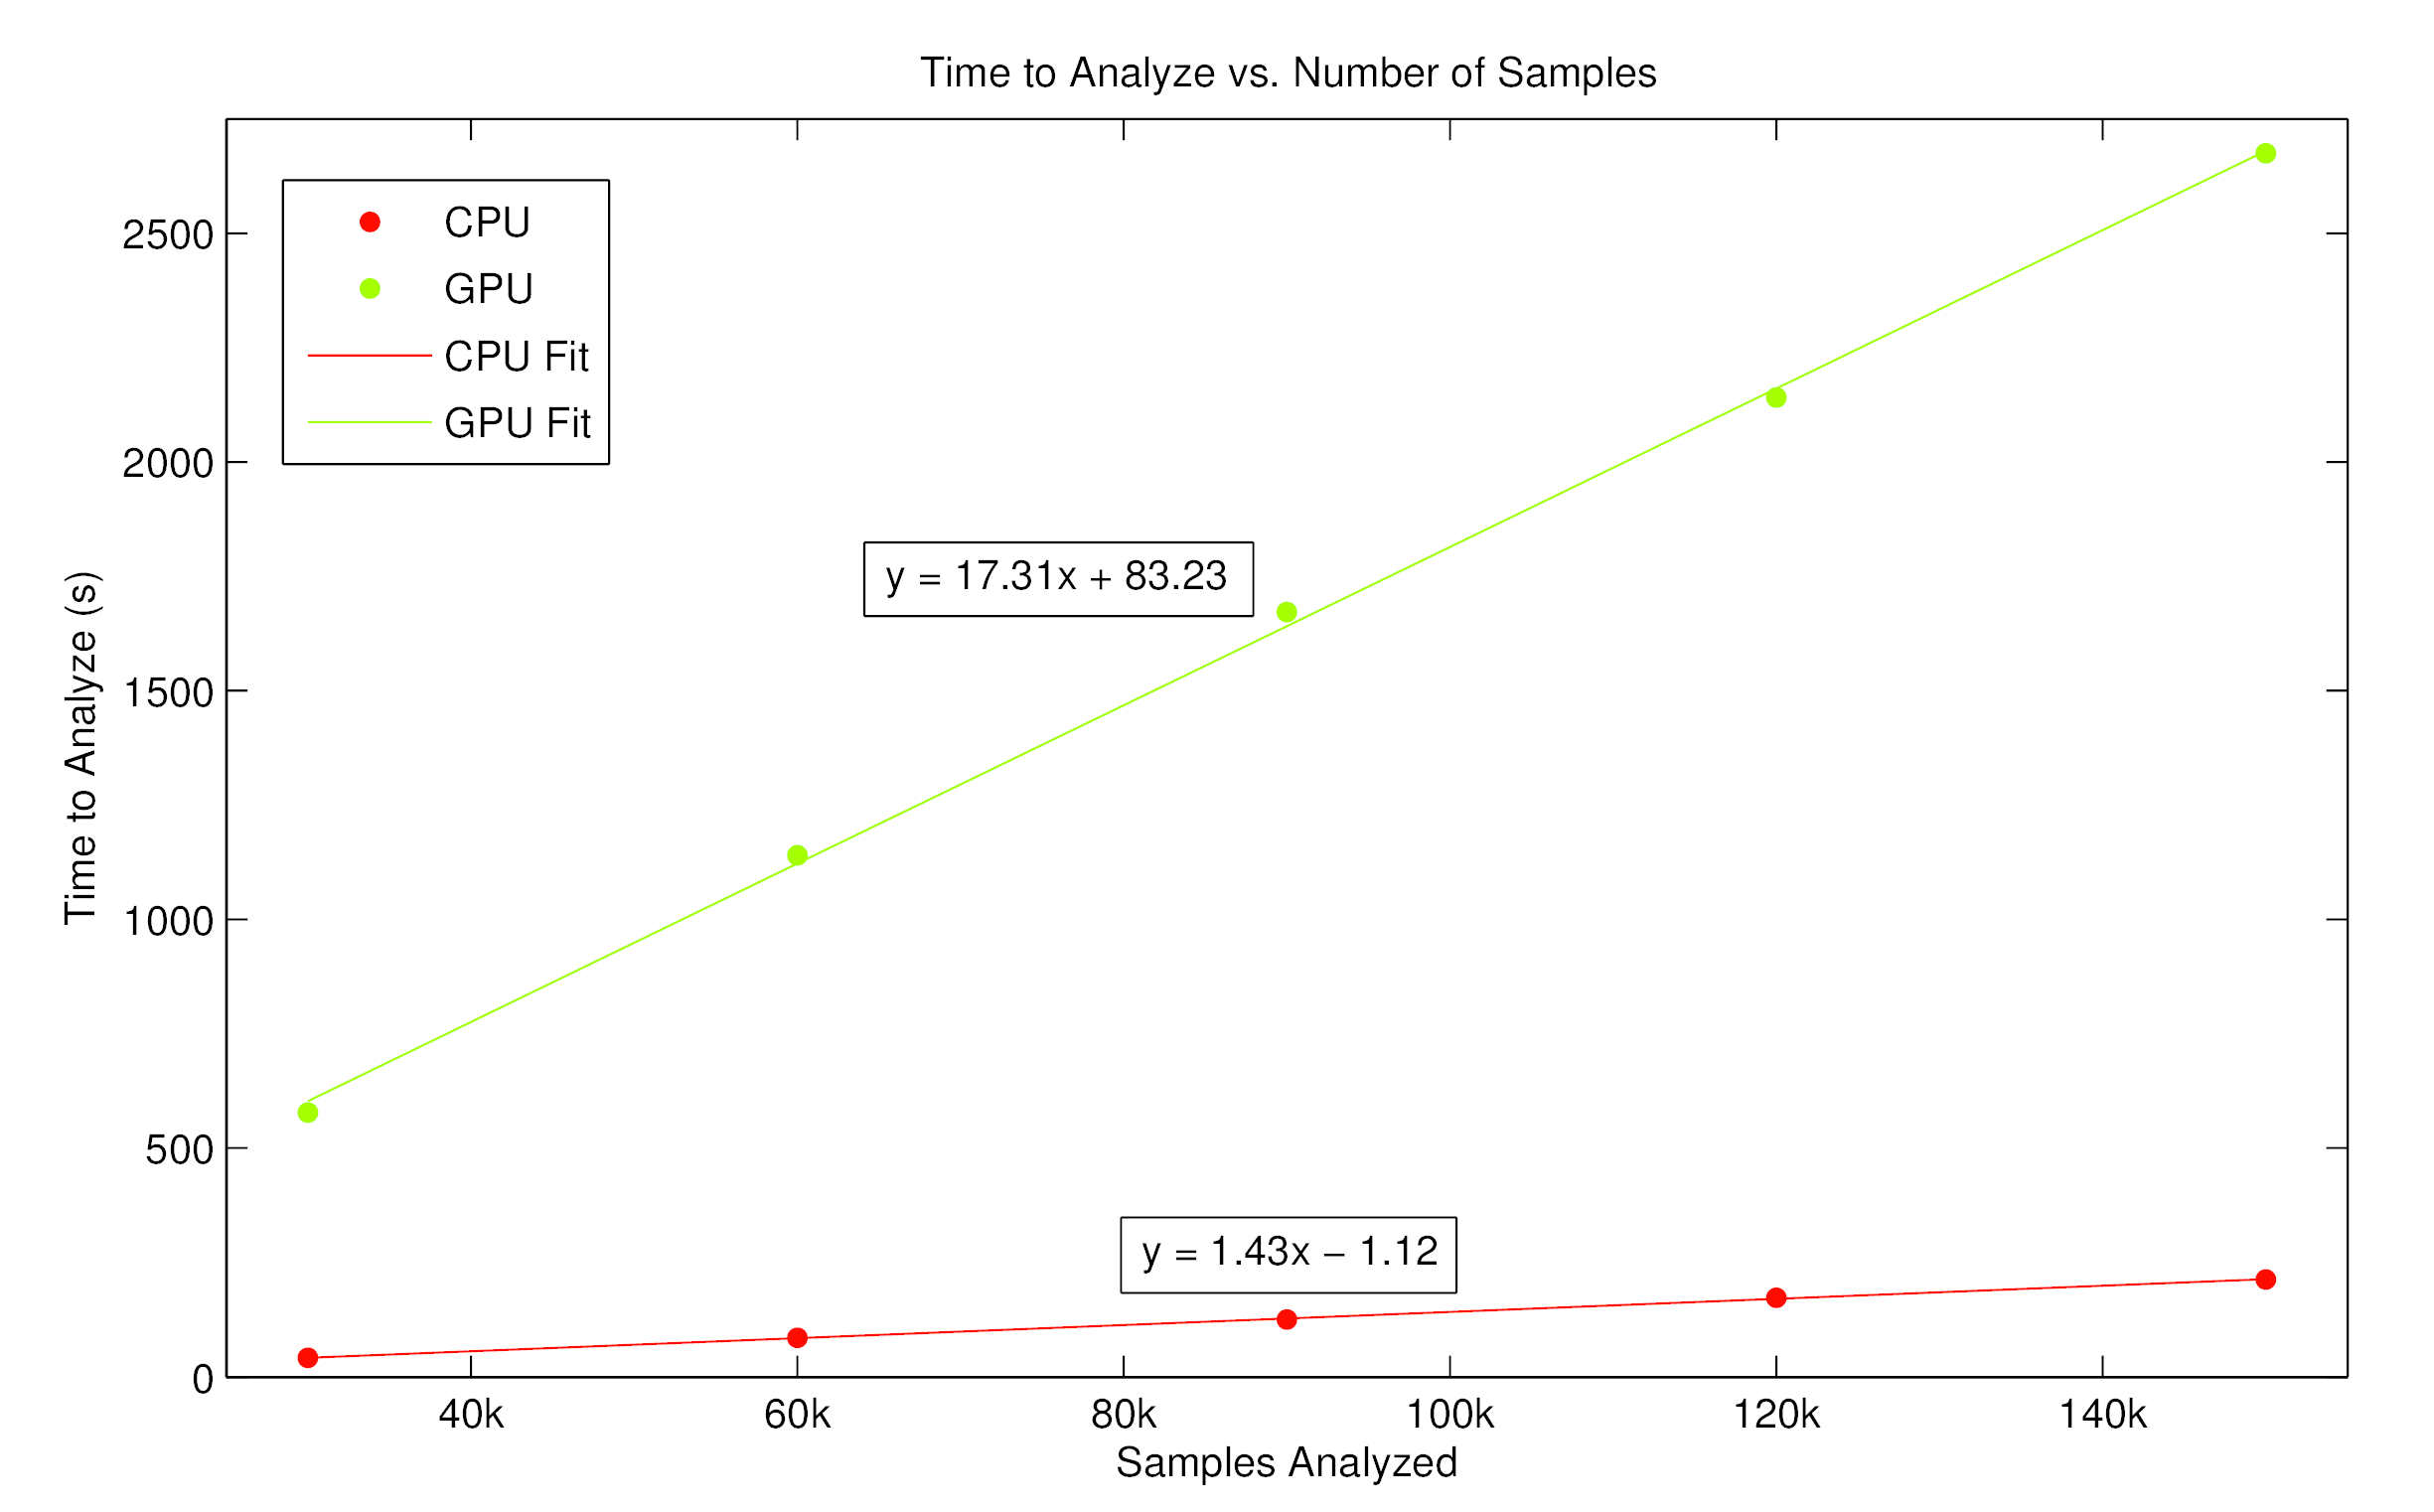
\includegraphics[width=0.6\paperwidth]{Time_vs_Samples.png}
    \caption{Plot of performance based on sample size, with a basis size of 30}
	\label{fig:samples}
\end{figure}

To demonstrate the impact of sample scaling with a larger basis size we ran a similar experiment using the largest basis size, the results of which are shown in Figure \ref{fig:samples:large}. For this experiment we used sample sizes of $10,000$, $20,000$, and $30,000$. Once again we trained an agent using both the GPU implementation and the CPU implementation. We observed that with a basis size of $258$ the GPU outperforms the CPU and appears to scale better. This change suggests that the effects of basis size and sample size on the performance scaling of LSPI are more complex than originally assumed and would benefit from further experimentation.

\begin{figure}%
    \centering
    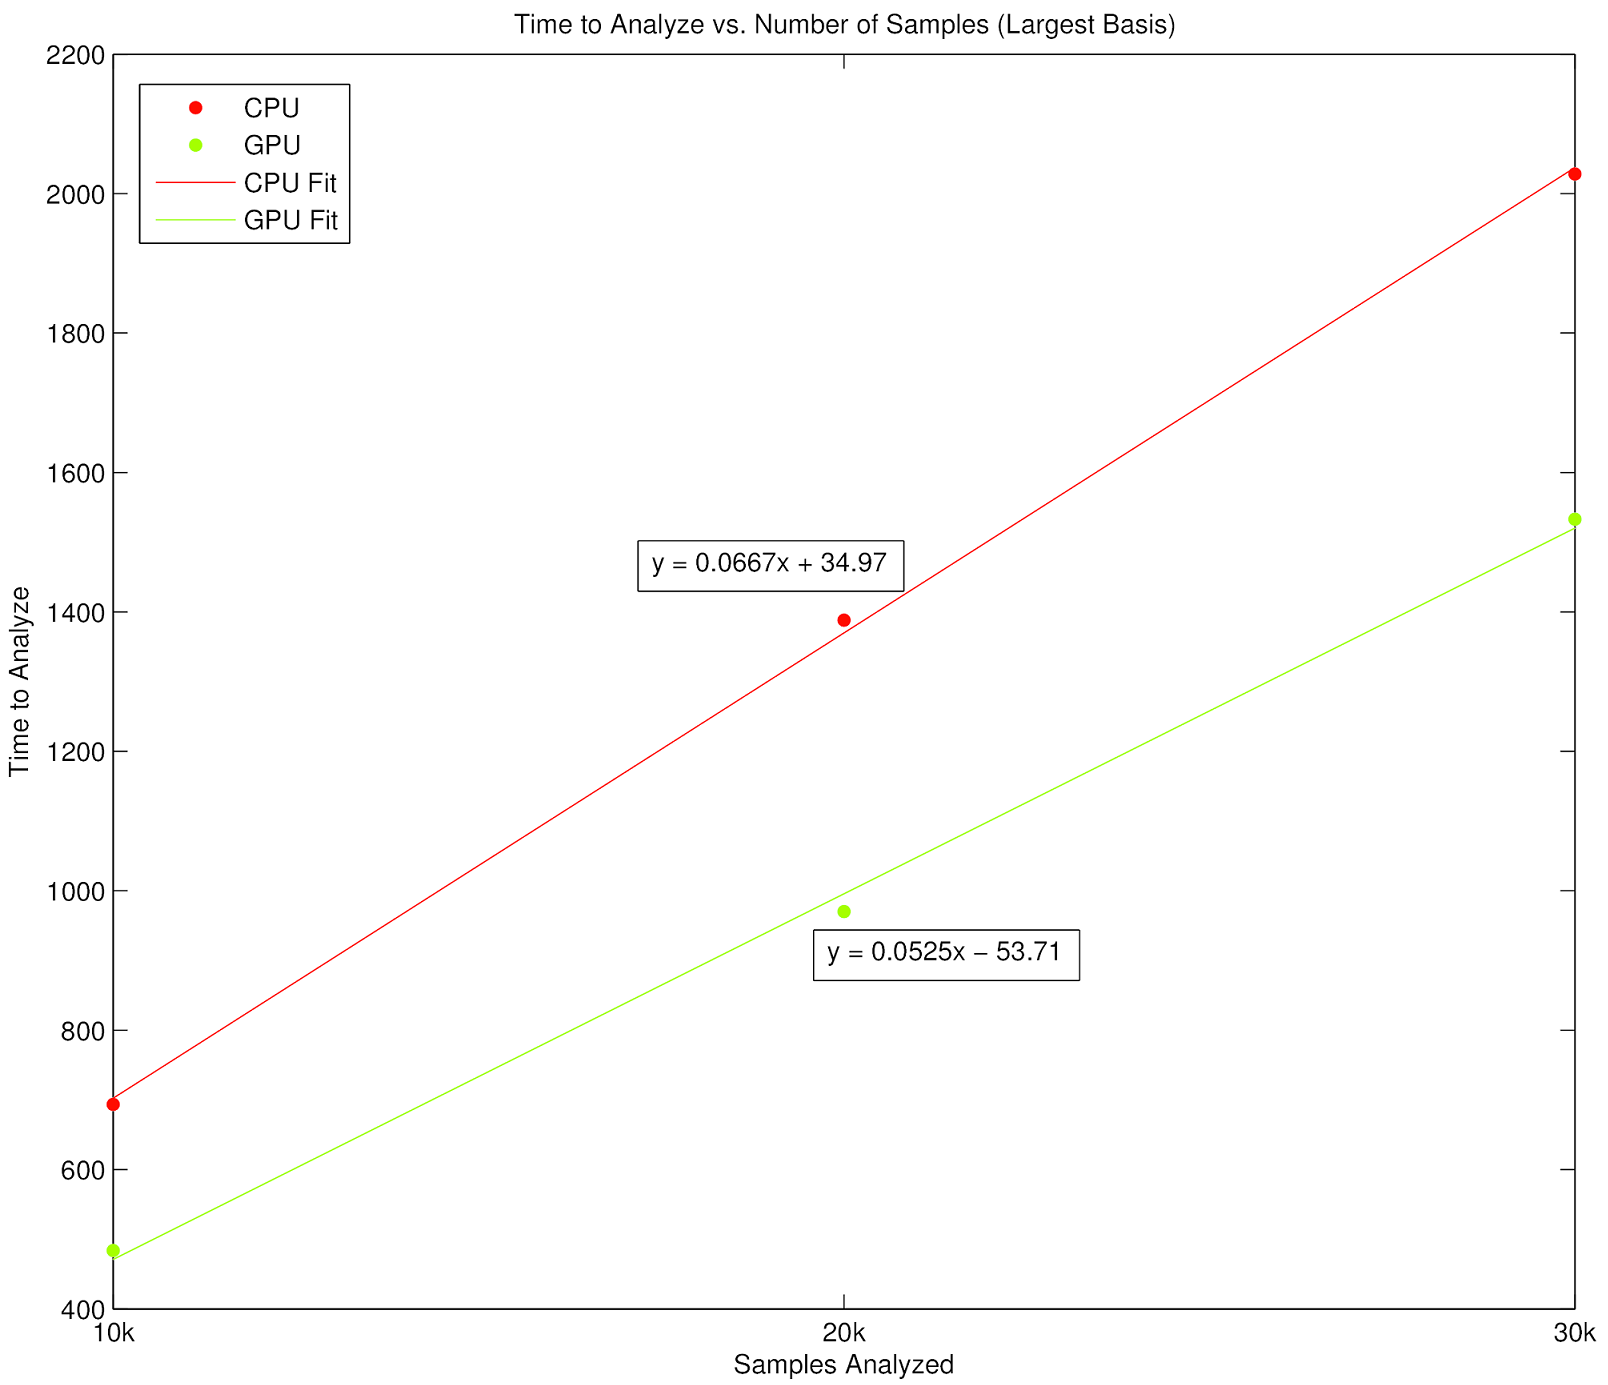
\includegraphics[height=0.4\paperheight]{Large_Time_vs_Samples.png}%
    \caption{Plot of performance based on sample size, with a basis size of 258}%
    \label{fig:samples:large}%
\end{figure}

The second experiment tested the performance of LSPI with a constant number of samples while the basis size increased. The experiment was setup by collecting $10,000$ samples from an agent following an arbitrary fixed policy with a $25\%$ exploration rate. These samples were then used to train agents with basis functions which ranged in size from $30$ to $258$. As with the samples scaling experiment, every attempt was made to ensure these experiments were completed in identical environments. Due to the variance we witnessed in our experiments we repeated this training for each agent three times for both the CPU and GPU implementation. The results are graphed with fit lines in Figure \ref{fig:basis}.

\begin{figure}
    \centering
    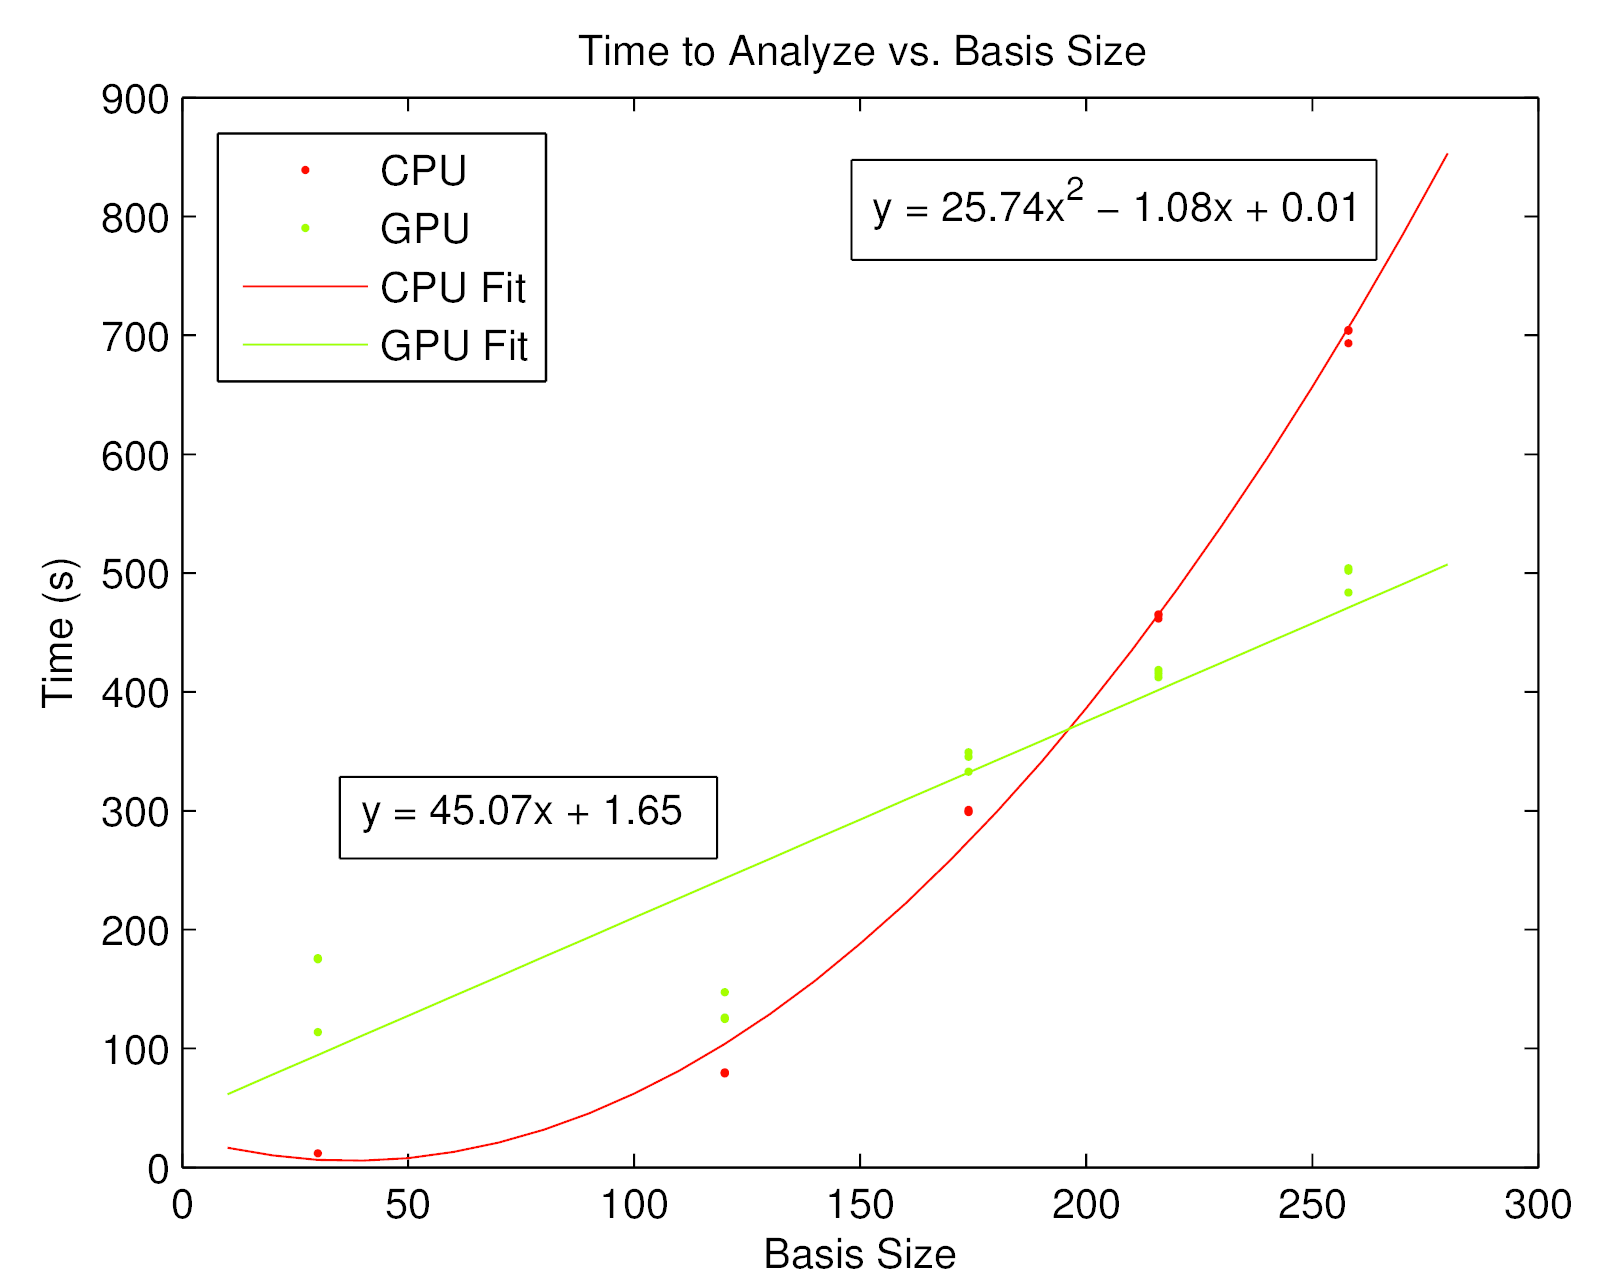
\includegraphics[height=0.33\paperheight]{Time_vs_Basis.png}
    \caption{Plot of performance based on basis size}
    \label{fig:basis}
\end{figure}

Based on the data we collected, it is clear that while the GPU performs slower than the CPU with small basis sizes, the GPU scales well with increasing basis size. For our particular configuration the performance crossover occurs around $200$; however, that intersection point will vary based on the specific hardware configurations as well as the optimizations used to improve performance and the number of samples used.

While the speeds we measured on the CPU were relatively stable, we noticed a high level of variance in our measurements for the GPU. Based on our knowledge of how linear algebra operations scale on the GPU, we would expect LSPI to scale approximately linearly on the GPU. Most of our data supports this; however, there are some outliers present on the graph.

When we measured the time to analyze the samples using a basis size of $120$ we were consistently seeing results that were comparable to the amount of time needed to analyze the samples using a basis of size $30$. To understand this result, we must first understand what factors will impact the amount of time needed to execute LSPI.

At its core, LSPI can be viewed as an optimization algorithm which iteratively executes the algorithm LSTD$Q$ in an attempt to locate the policy which maximizes the utility of the agent for the given samples. Depending on both the samples and the basis function used to evaluate the samples, the number of iterations of LSTD$Q$ necessary can change. Looking at Figure \ref{fig:basis} the data shows that although it is less noticeable, all three tests for the CPU also appear under the curve. This suggests that the particular features we selected may have had an impact on the number of iterations of LSTD$Q$ required to converge.

Another potential contributing factor to this result is the nature of the GPU architecture. When code is executed on the GPU, some number of processing units is allocated. The number of processing units allocated does not necessarily correspond with the size of the data input. As a result, there may be processing units which are effectively idle. The end result is that two operations with different input sizes may take the same amount of time. Between the architecture of the GPU and the interaction of the basis features with the speed of convergence, we feel that these results still fall within the expected range.

When it came time to plot fit lines for the data, the choice was obvious for the CPU: the results very clearly represent a second degree polynomial, with $R^2 = 0.99$. For the GPU the choice was less obvious, particularly since the outlier at $120$ made any fit difficult. We chose a linear fit because the data fits a linear model better with the outliers removed. The fit was less consistent for the GPU data with $R^2 = 0.7987$.

It is important to keep in mind that the point at which the GPU overtakes the CPU in performance will vary based on specific hardware configurations, as well as the level of optimization put into the implementation. As stated earlier, we chose to optimize very little to focus on the scaling performance gains. Furthermore, unless the CPU implementation was capable of being optimized at a rate much higher than the GPU optimizations, these performance tweaks would only serve to lower the barrier for seeing improvements with the GPU.

In our experiments we were able to generate very good policies with a very small basis function; however, this is largely due to the amount of hand written scripts our bot relies on to interact with the environment. While this allowed us to test the performance of LSPI under different conditions very well, our AI implementation does not do allow more complex behavior to be learned, limiting the benefits observed using reinforcement learning.

To intuitively understand the benefits of a large basis function, consider designing an AI agent for Quake III from the ground up. In order to manage the complexity of the environment, it is helpful to have some basic actions available to the agent: \emph{attack}, \emph{get health}, \emph{get weapon}, \emph{get armor}, \emph{get powerup}, \emph{search for enemy}, \emph{defend location}, \emph{flee from enemy}, \emph{change weapon}, \emph{reload}. Already our agent has more actions available than the implementation was used for testing.

Now consider what information would be useful in order to make intelligent decisions. First and foremost, the agent needs information on its own state: \emph{health}, \emph{armor}, \emph{equipped weapon}, \emph{available weapons}, \emph{equipped ammo}, \emph{available ammo}. Keep in mind that some of these features, such as equipped weapon and available weapons, would need to be represented by multiple values in the basis. In fact, representing this information in Quake III would already result in a basis with $23$ values which must be repeated for each of the $10$ actions we have defined for a total size of $230$, and we still lack the information to make more complex decisions such as how to choose an area to defend.

\subsection{Impact of Increasing Basis Size}

To empirically demonstrate the impact of increasing the basis size we used an LSPI agent to solve the \emph{inverted pendulum} problem. The problem requires an agent to balance an inverted pendulum attached to a cart by applying one of three actions: left force (-75 Newtons), right force (75 Newtons), or no force (0 Newtons). All actions have noise added uniformly from $-10$ to $10$. The state space is continuous and composed of the vertical angle $\theta$ and the angular velocity $\dot{\theta}$ of the pendulum. The transitions are governed by the following equation \cite{lspi}:

\begin{equation}
    \ddot{\theta} = \frac{g sin(\theta) 0 \alpha ml(\dot{\theta})^2 sin(2\theta)/2 - \alpha cos(\theta)u}{4l/3 - \alpha ml cos^2(\theta)}
\label{eq:pendulum}
\end{equation}
where $g$ represents the gravity constant, $m$ is the pendulum mass, $M$ is the cart mass, $l$ is the pendulum length, $\alpha = 1/(m + M)$, and $u$ is the noisy input. The simulation steps every 0.1 seconds, selecting the agent's action at the beginning of the step and keeping it constant until the next action is selected. If $|\theta| \geq \pi/2$ the pendulum is considered horizontal and receives a reward of $-1$, otherwise the agent receives a reward of 0.

For our test we used the following values:
\[
    \begin{aligned}
        g &= 29.4 m/s^2 \\
        m &= 2.0 kg \\
        M &= 8.0 kg \\
        l &= 3.0 m
    \end{aligned}
\]
and a discount factor of 0.95. The basis function was created by generating $N$ Gaussian functions arranged over the 2-dimensional state space and including a constant factor of $1$. For state $s = (\theta,\dot{\theta})$ and some action $a$, all values are $0$ except for the active block for $a$ which is represented by:
\[
    \big(1, e^{-\frac{||s - \mu_1||^2}{2\sigma^2}}, e^{-\frac{||s - \mu_2||^2}{2\sigma^2}}, \dots, e^{-\frac{||s - \mu_N||^2}{2\sigma^2}}\big)^T
\]
where $\mu_i$ represents a point in the space $\theta \times \dot{\theta}$ and $\sigma^2 = 1$. Specifically, the values for $\mu$ were selected by choosing $N$ uniformly spaced discrete pairs $(\theta, \dot{\theta})$ such that $\theta \in [-\pi/2, \pi/2]$ and $\dot{\theta} \in [-1, 1]$. 

Training samples were collected from random episodes: the pendulum started at a position near $(0,0)$ and the agent selected actions at random. The average length of each episode was 16, generating about 16 samples. Figure \ref{fig:pendulum} shows the performance of policies created for varying number of training episodes.

\begin{figure}
	\centering
		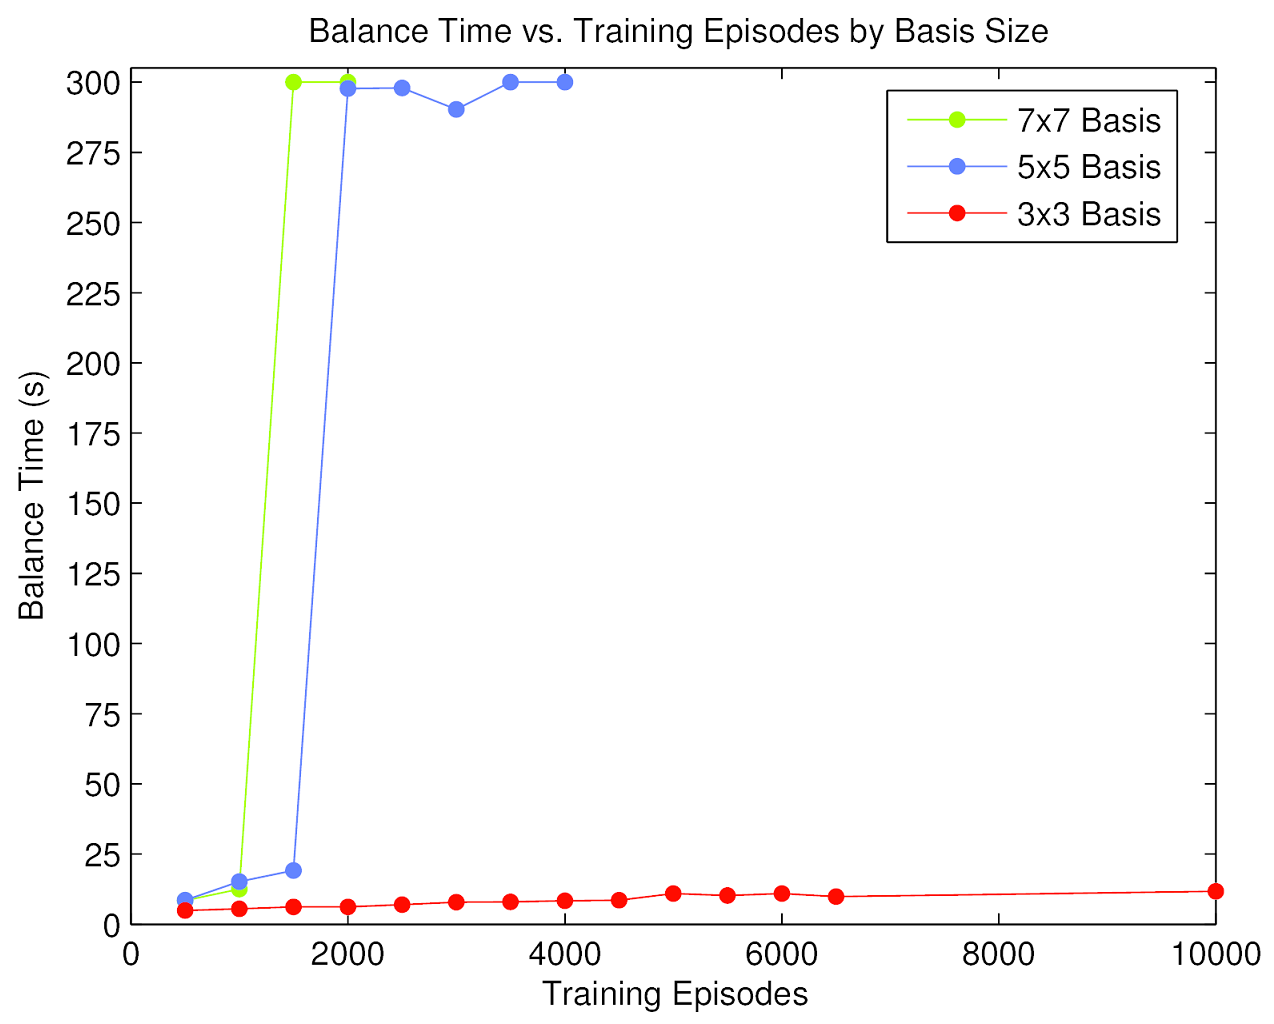
\includegraphics[width=0.33\paperheight]{Balance_vs_Samples.png}
	\label{fig:pendulum}
    \caption{LSPI Inverted Pendulum: Average balancing time}
\end{figure}

If the agent balances for $300$ seconds the episode comes to an end as it is likely the agent has developed an optimal policy. For each basis size we increased the number of training episodes by $500$ until two perfect results were achieved. The smallest basis was tested up $6.5$k training samples before we skipped to $10$k and then $15$k (not shown). None of these tests showed any significant improvement so we discontinued testing.

The numbers in the legend of Figure \ref{fig:pendulum} lists the basis size in terms of the number of discrete values for $\theta$ and $\dot{\theta}$ selected from. For example the smallest basis size was created by selecting points from $\{-\pi/2, 0, \pi/2\} \times \{-1, 0, 1\}$.

The experiment results demonstrate that the size of the basis function can have an impact on two important convergence factors. First, the smallest basis function did not contain enough information to converge on an optimal solution, suggesting that a larger basis function may be required in order to implement an effective agent. Second, the largest basis function needed fewer samples to converge when compared to the medium basis function. In some environments this may provide a performance benefit while in others it is desirable because the agent can learn effective policies with less training time.

\section{Semi-Online LSPI}

The algorithm for Semi-Online LSPI is described in Section \ref{chap:implementation:lspi}. To evaluate its effectiveness as an alternative to traditional online algorithms we implemented OLPOMDP and Semi-Online LSPI in the Quake III environment and compared their performance and effectiveness.

\subsection{Policy Gradient}

The term \emph{Policy Gradient} describes a class of machine learning techniques which apply gradient ascent optimization to determine the optimal policy. Given the policy value function, $p(\theta)$, policy gradient algorithms can be succinctly described by the following formula:

\[
    \theta_{n+1} = \theta_{n} + \alpha\nabla_\theta p(\theta_{n})
\]
where $\theta$ represents the policy parameters and $\alpha$ is referred to as the step size or learning rate \cite{norvig}\cite{bishop}.

Before we estimate $\nabla_\theta p(\theta)$, we must ensure that $p(\theta)$ is differentiable with respect to $\theta$. Assume we have a basis function, $J_\theta(s,a)$ which is used to generate a policy as follows:

\[
    \pi_\theta(s,a) = \argmax_a J_\theta(s,a)
\]
The use of the $argmax$ function may result in a discontinuous distribution. This can be fixed by using a probabilistic policy \cite{olpomdp:lecture}:

\begin{equation}
\label{eq:grad:policy}
    \pi_\theta(s,a) = Pr(a|s) = \frac{e^{J_\theta(s,a)/T}}{\sum\limits_{a'\in A} e^{J_\theta(s,a')/T}}
\end{equation}

To estimate the gradient from samples we use the following formula:
\begin{equation}
\label{eq:grad}
    \begin{aligned}
        \nabla_\theta p(\theta) &= \sum_a\pi_\theta(s_0,a)g_\theta(s_0,a)R(a) \\
        g_\theta(s_0,a) &= f_\theta(s_0, a) - \sum\limits_{a'} \pi_\theta(s_0,a')f_\theta(s_0,a')
    \end{aligned}
\end{equation}

Equation \ref{eq:grad} is the basis for an online algorithm called OLPOMDP \cite{olpomdp}. Intuitively, the algorithm estimates the gradient using Monte Carlo techniques: execute the policy while making small changes to $\theta$. Because we use Equation \ref{eq:grad:policy} to select actions, our agent will naturally explore the environment. With each action we then update the value $e$, called the eligibility trace, by estimating the value of the gradient for that action.

The pseudocode for OLPOMDP is given in Algorithm \ref{olpomdp}. Notice that instead of updating $\theta$ directly the value $e$, called the eligibility trace, is used as an intermediary. The eligibility trace represents the discounted sum of gradients over previous state-action pairs and is used to update $\theta$ according to the reward given for the corresponding action. The value $\beta$ is referred to as the bias and controls the weight of previous experiences in the environment. Increasing $\beta$ biases the algorithm toward past experiences while also increasing the variance. 

\begin{algorithm}
\caption{OLPOMDP}
\label{olpomdp}
    {\fontsize{12}{10}\selectfont
    \begin{algorithmic}[1]
        \REQUIRE
            \begin{itemize} 
                \item $\beta \in [0,1)$ 
                \item $T > 0$ 
                \item $\theta_0 \in \mathbb{R}^K$ 
            \end{itemize}
    \STATE Set $e = 0$
    \FOR{$t = 0$ to $\infty$}
        \STATE Observe the current state, $s$
        \STATE Select action $a$ according to $\pi_\theta(s)$
        \STATE Execute $a$
        \STATE Observe reward $r$
        \STATE $e \leftarrow \beta e + f(s,a) - \sum\limits_{a'}\pi_\theta(s,a')f_\theta(s,a')$
        \STATE $\theta \leftarrow + \alpha \cdot r \cdot e$
    \ENDFOR
    \end{algorithmic}
    }
\end{algorithm}

\subsection{Evaluation of Online Algorithms}

For the purpose of comparison both agents were tested using GPU acceleration in identically configured Quake III matches. All bots were given the personality of \emph{Ranger} to ensure no bots, including the Quake III bots, had any unfair advantages in physical characteristics. We evaluated the performance of each agent in a deathmatch against a native bot with no time limit and a 500 kill limit. The difficulty was set to \emph{Bring It On}, the second lowest difficulty level. This provided us the benefit of creating a high contrast between good and bad policies due to the impact on scripted bot behavior. The Online LSPI agent used a discount rate of $0.95$ and an exploration rate of $0.25$. The OLPOMDP agent used $\beta = 0.80$ and a step size of $0.05$. To increase the rate of updates for Online LSPI we appended samples collected from the agent's policy as well. This increased the sampling bias and may have impacted our results; however, the effect is likely small due to the relatively small number of samples needed to generate good policies.

\begin{figure}
		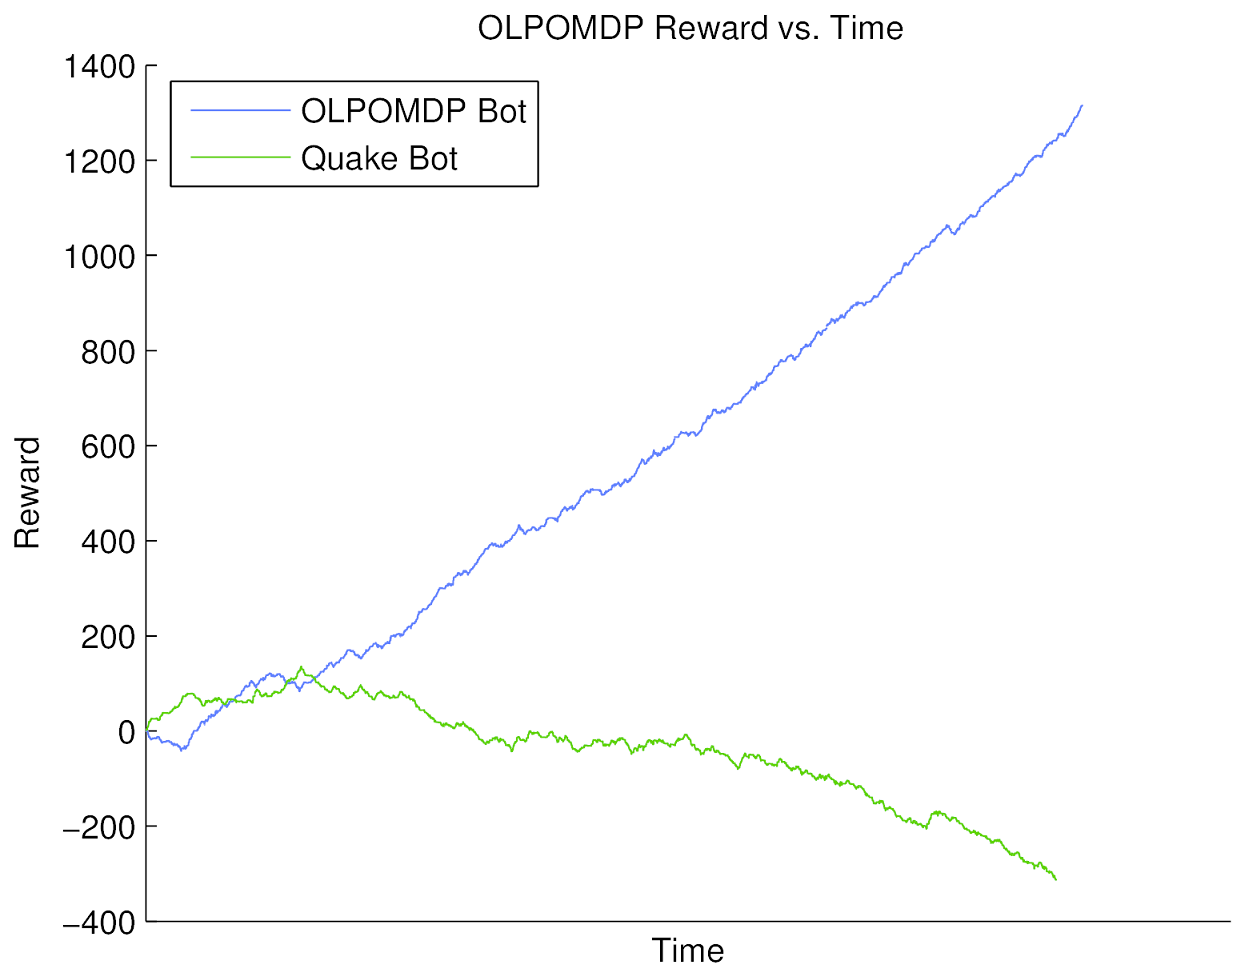
\includegraphics[width=0.5\textwidth]{OLPOMDP_Reward_vs_Time.png}
        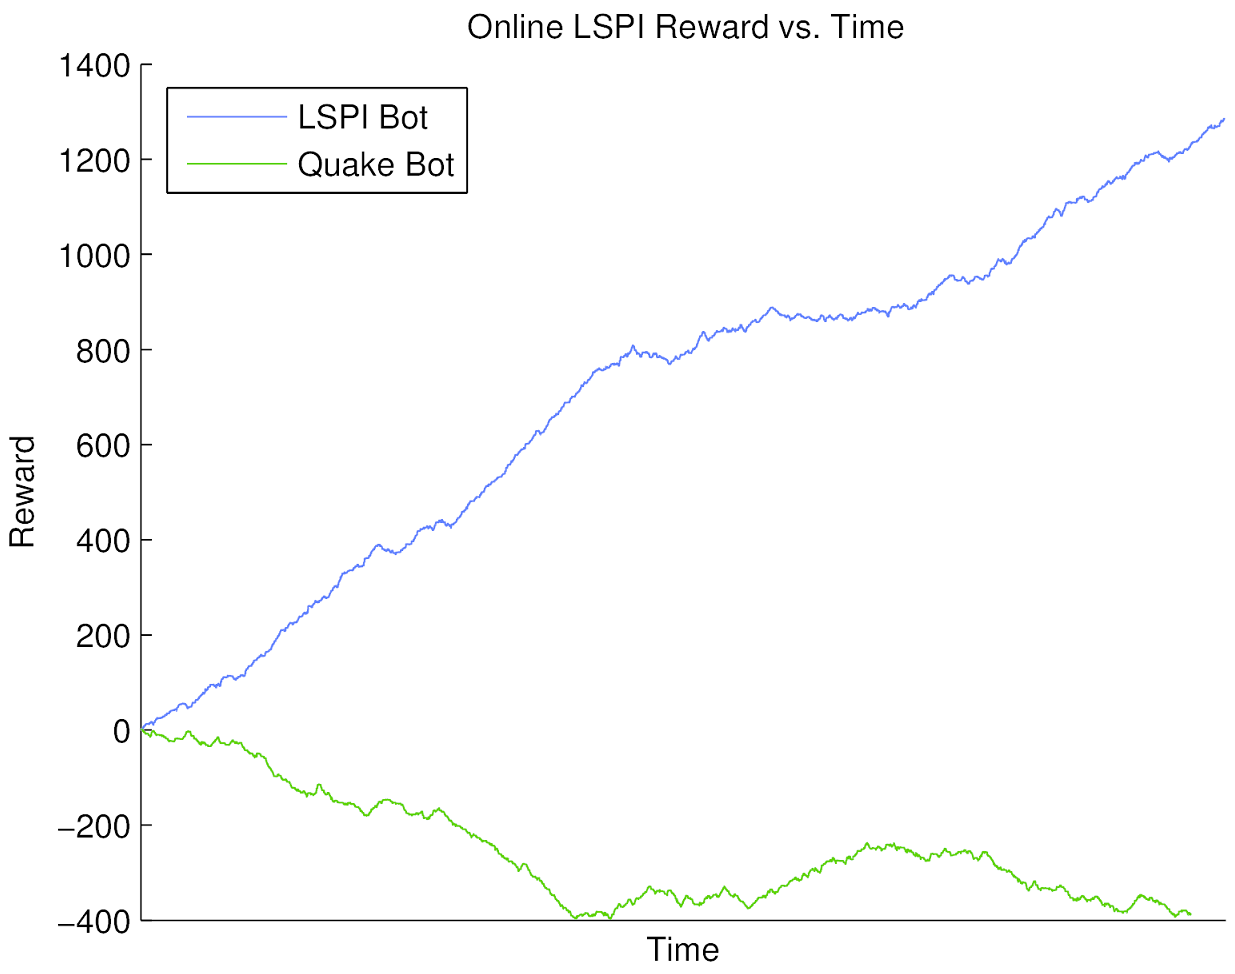
\includegraphics[width=0.5\textwidth]{LSPI_Reward_vs_Time.png}
	\label{fig:online:reward}
    \caption{Online Agent Reward}
\end{figure}

The result of the matches is displayed in Figure \ref{fig:online:reward}. Both the Online LSPI and OLPOMDP agents were able to win when placed against the native bot. In both matches our agents scored approximately twice as many kills as the native bots. While the end result was the same, a few differences are noticeable in the reward graphs. The LSPI agent appeared to start with a better policy, although the OLPOMDP agent was quickly able to overcome this advantage and finish the match with a reward of $1316$ as compared to the LSPI agent with $1286$. In addition, OLPOMDP demonstrated a more stable average reward with the policy changes in LSPI appearing to cause some reward loss. Overall, however, both algorithms performed on par and achieved nearly the same end result.

\begin{figure}
	\centering
		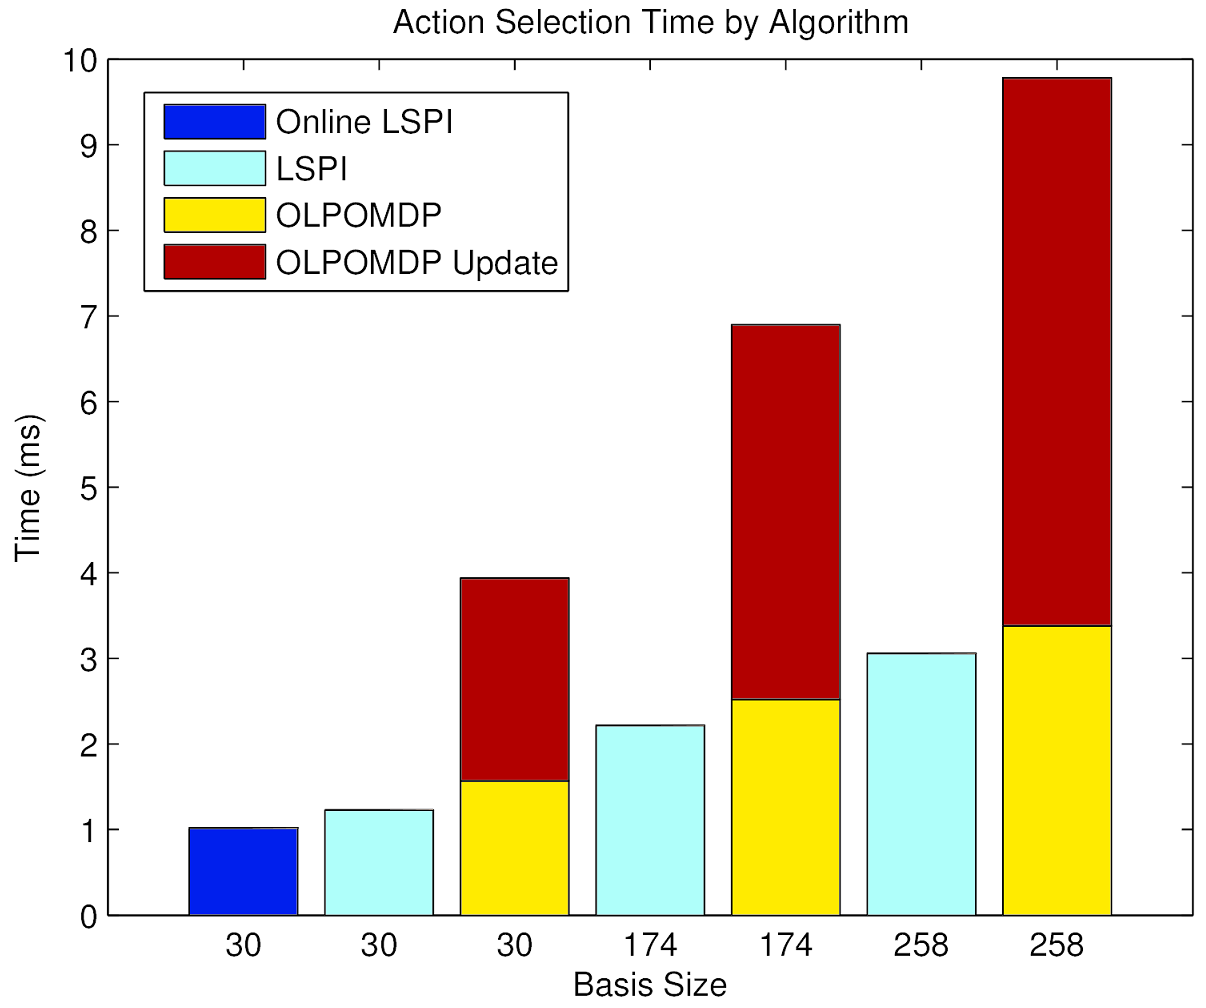
\includegraphics[height=0.33\paperheight]{Action_Selection_Time.png}
	\caption{Average time required to select an action.}
	\label{fig:action:selection}
\end{figure}

Figure \ref{fig:action:selection} shows the average time required to select an action for each agent across the small, medium, and large basis sizes. The values for LSPI and OLPOMDP were selected by tracking the amount of time each action selection operation took over the course of a deathmatch to $50$. The value for Online LSPI was taken from the experiment demonstrated in Figure \ref{fig:online:reward}. For clarity the values for OLPOMDP were split into the update and action selection steps.

We observed that Online LSPI does not appear to suffer any performance loss due to the background updates. To understand this result, recall that GPU operations are generally bound by memory operations. In order to reduce the impact of delays waiting for memory operations to complete the hardware is optimized for fast context switching, allowing multiple programs or operations to interleave rapidly \cite{gpgpu}. 

Because we did not optimize our code to minimize the delay in memory, we do not appear to lose performance when we add simultaneous operations. Note, however, that if we were to optimize all operations it is possible that LSPI would begin to perform better as we approach the GPU's throughput limit. It is also possible that the exploration policy for Semi-Online LSPI improved performance over LSPI because the basis function does not need to be computed when a random action is selected.

We observed approximately a factor of 4 speedup when using Online LSPI over OLPOMDP. OLPOMDP appears to be dominated by the update step, which consistently takes longer than just selecting an action; however, action selection also takes slightly longer due to the requirement to generate random numbers to follow the probabilistic policy.

\begin{figure}
	\centering
		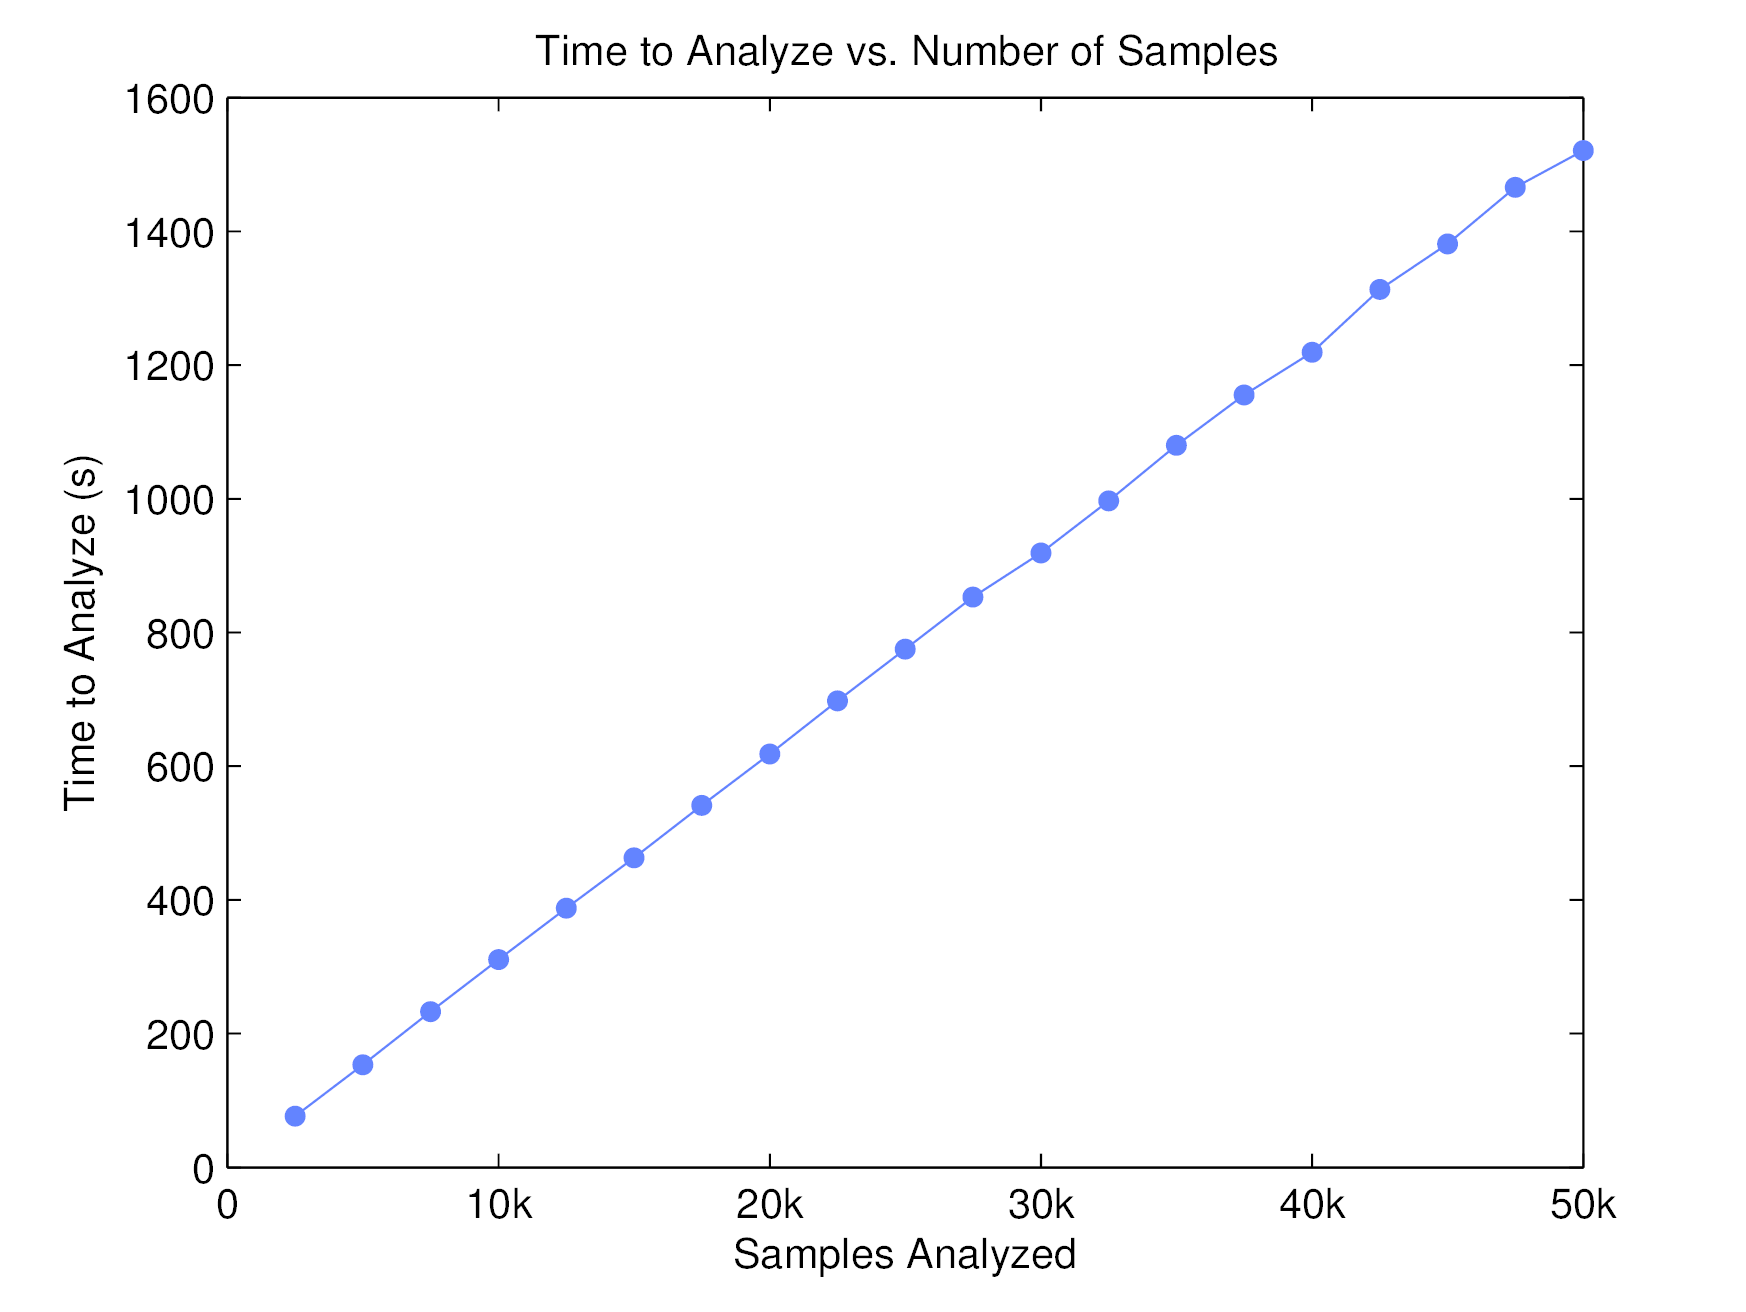
\includegraphics[height=0.33\paperheight]{Online_Time_vs_Samples.png}
	\caption{Time to analyze samples in Online LSPI.}
	\label{fig:online:samples}
\end{figure}

The results in Figure \ref{fig:online:samples} demonstrate the scaling of analysis as samples are collected in Online LSPI. We chose not to directly include the results from Figure \ref{fig:samples}, as they cannot be directly compared. For the sample scaling tests, the samples included the time to load the samples from a file, but in this test the samples were already in memory. Despite this disparity, our test clearly demonstrates no significant performance loss when running online with a speed improvement of $20\%$ over our previous tests and approximately the same scaling factor. Accounting for the file operations it appears that our experiment performed almost identically in online and offline mode. It is worth noting that in a more taxing graphical environment less computing power would be available and we would expect to start seeing performance losses.

Our results indicate that LSPI is capable of learning good policies in an FPS environment, LSPI scales better with larger basis functions when using the GPU, and it is possible to update an agent's policy using LSPI in a semi-online manner without a significant loss of performance.
	\chapter{Results}
	
	

	\bibliography{refs}
\end{document}